%-------------------BASICS-------------------
\documentclass[oneside,final,12pt]{article} %одностороння печать, чистовая версия, размер кегля, класс документа
\usepackage{ucs} 
\usepackage[utf8x]{inputenc} 
\usepackage[T2A, T1]{fontenc} 
\usepackage[english,russian]{babel} %оформление кириллицей (подписи к таблицам и т.д.)
\usepackage{ifpdf}
\ifpdf  %% если используется pdfTEX
\usepackage{cmap}  %поиск по кириллице в готовом pdf
\usepackage[pdftex]{graphicx} %работа с графикой 
\usepackage[unicode=true]{hyperref}
\usepackage{pdfpages}
\else   %% если используется не pdfTEX
\usepackage[dvips]{graphicx}
\fi
\usepackage{verbatim} %comments
\setcounter{tocdepth}{2} % глубина содержания
 
 
%-------------------FORMAT-------------------
\usepackage{vmargin} %размеры полос набора
\setpapersize{A4} %формат бумаги
\setmarginsrb{20mm}{20mm}{20mm}{20mm}{0pt}{0mm}{0pt}{13mm} %размеры полей: левое, верхнее, правое, нижнее, 3*колонтитулы, расстояние между нижним краем нижней строки и нижним краем номера страницы
\usepackage{indentfirst} %красная строка для первого абзаца главы или параграфа
\setlength{\parindent}{0cm} % отступ красной строки
\setlength{\parskip}{2mm}
\sloppy %борьба с залезанием строк на поля путём изменения размеров пробелов
\pagestyle{plain} %включена нумерация страниц 
\renewcommand{\thesection}{\arabic{section}}  %арабская нумерация глав
\usepackage{lineno} %нумерация всех строк для отладки
\usepackage{enumitem} %особенности enumerate
\usepackage{textgreek} % \textalpha греческие буквы не в math mode
\usepackage{setspace} %for setstretch
\usepackage{adjustbox}
\usepackage{rotating}
\usepackage{lscape} 

%-------------------TABLES, FIGURES-------------------
\usepackage{float} %для плавающих картинок и таблиц
%\usepackage{wrapfig} %для плавающих картинок.
\usepackage[font=small]{caption}
\usepackage{booktabs} %отступы в tabular
\usepackage{colortbl} %раскаршивание таблиц
\usepackage{xcolor} %название цветов
\newcommand{\red}[1]{\textcolor{red}{#1}} % выделение красным текста командой \red{}

\definecolor{dark-dark-gray}{gray}{0.3}
\newcommand{\gray}[1]{\textcolor{dark-dark-gray}{#1}}
\definecolor{dark-gray}{gray}{0.4}
\newcommand{\graytable}[0]{\arrayrulecolor{dark-gray}}
\newcommand{\thinrule}[0]{\specialrule{0.3pt}{4pt}{4pt}}
\newcommand{\verythinrule}[0]{\specialrule{0.1pt}{1pt}{1pt}}
\newcommand{\invisiblerule}[0]{\specialrule{0pt}{2pt}{2pt}}

\usepackage{pbox} % для переносов внутри ячейки таблицы
\usepackage{array} %??
\usepackage{longtable}% перенос таблиц на страницах
\usepackage{subcaption} % несколько картинок в одной
\usepackage{multirow} % объединение ячеек
\newcolumntype{R}[1]{>{\raggedleft\arraybackslash}p{#1}}
\usepackage{tabu}

\usepackage{caption}
\captionsetup{%
    ,format=hang
    ,justification=raggedright
    ,singlelinecheck=false
    ,figureposition=bottom
    }

\usepackage{tikz}
\usetikzlibrary{shapes.geometric,shapes.arrows,decorations.pathmorphing}
\usetikzlibrary{matrix,chains,scopes,positioning,arrows,fit}


%-------------------MATH-------------------
\usepackage{amsmath} %дополнительные средства для вёрстки формул
\everymath{\displaystyle}
\usepackage{breqn} %для dmath разбить длинную формулу
%\usepackage{esvect} %vectors

%\usepackage{amscd} %диаграммы
\usepackage{amsfonts} %дополнительные шрифты для формул
\usepackage{amssymb} %дополнительные символы для формул

%-------------------BIBLIOGRAPHY-------------------
\usepackage{cite}
\usepackage[nottoc,notlot,notlof]{tocbibind}


\begin{document}
		%\linenumbers
		\tikzstyle{line}=[thick, ->]
\tikzstyle{dnn}=[draw, circle, minimum width=1cm]

\newcommand{\ohe}[3]{
	\def\step{0.2}
	\def\hlen{#3}
	\foreach \x in {0,...,4}
	\draw[] (#1-\hlen*\step, #2-\step*\x) -- (#1+\hlen*\step,#2-\step*\x);
	
	\foreach \x in {-\hlen,...,\hlen}
		\draw (#1-\step*\x, #2) -- (#1-\step*\x, #2-4*\step); 
	}
	
\newcommand{\oherandom}[4]{
	\def\step{0.2}
	\def\len{#3}
	\def\depth{#4}
	\foreach \x in {0,...,\depth}
	\draw[] (#1-\len*\step*0.5, #2-\step*\x) -- (#1+\len*\step*0.5, #2-\step*\x);
	
	\foreach \x in {0,...,\len}
		\draw (#1+\step*\x-\len*\step*0.5, #2) -- (#1+\step*\x - \len*\step*0.5, #2-\depth*\step); 
	}	
	
	
\newcommand{\flattenout}[3]{
	\def\step{0.1}
	\def\lenflat{#3}
	
	\foreach \x in {0, 1}
	\draw[] (#1-\lenflat*\step*0.5, #2-\step*\x) -- (#1+\lenflat*\step*0.5,#2-\step*\x);
	\foreach \x in {0,...,\lenflat}
		\draw (#1+\step*\x -\lenflat*\step*0.5, #2) -- (#1+\step*\x -\lenflat*\step*0.5, #2-\step);
	}

\newcommand{\out}[2]{
	\def\step{0.5}
	\foreach \x in {0, 1}
		\draw[] (#1-\step*2, #2-\step*\x) -- (#1+\step*2,#2-\step*\x);
	\foreach \x in {-2,...,2}
		\draw (#1+\step*\x, #2) -- (#1+\step*\x, #2-\step); 
	\node[inner sep=0] (out0) at (#1-1.5*\step, #2) {};
	\node[inner sep=0] (out1) at (#1-0.5*\step, #2) {};
	\node[inner sep=0] (out2) at (#1+0.5*\step, #2) {};
	\node[inner sep=0] (out3) at (#1+1.5*\step, #2) {};
}

\tikzstyle{cnn}=[draw, rectangle, minimum height=2em, minimum width = 0.8em]	

%        \begin{titlepage}

\newcommand{\HRule}{\rule{\linewidth}{0.3mm}} % Defines a new command for the horizontal lines, change thickness here

\center

\textbf{\textsc{\Large московский государственный университет} \textsc{\large имени }\textsc{\Large М.В.Ломоносова}}
\\[0.3cm] 
\HRule 
\\[0.3cm]
\textbf{\textsc{\large факультет биоинженерии и биоинформатики}}
\\[4.0cm]

\begin{spacing}{1.4}
{ \LARGE \bfseries  Использование нейронных сетей в задачах предсказания нуклеотидных последовательностей}  \\[1.0cm] 


{\LARGE \bfseries The use of neural networks for nucleotide sequences prediction problems} \\[2.0cm] \end{spacing} 
 
 
\Large \emph{Курсовая работа студентки четвертого курса:}\\
Литвин Анны Валерьевны
\\[3cm]



\begin{flushright} \large
Научные руководители: \\
профессор,\,д.б.н.\,Гельфанд\,М.С.\\
аспирант\,Червонцева\,З.С.\\
\end{flushright}

%\begin{flushleft}\large
%\makebox[1.5in]{\hrulefill} 
%\end{flushleft}



\vfill

{\large Москва \\ 2019}
\end{titlepage}
 \newpage
%        \tableofcontents \newpage
        %\include{abbreviations} \newpage
%        \section{Введение}

С появлением первых секвенированных последовательностей генов и геномов появились попытки описать эти последовательности с помощью математических моделей.
Одни из первых моделей опирались на известные тогда вирусные геномы -- стационарная \cite{garden_markov_1980}, нестационарная Марковская модели \cite{tavare_codon_1989}, скрытые Марковский модели \cite{churchill_stochastic_1989}. 
Давно стало известно, что геномы про- и эукариот неравновесны по вхождениям ди-, три-, тетрануклеотидных последовательностей -- в общем случае k-меров \cite{phillips_mono-_1987}. 
Тем не менее, описать общую структуру генома, не вдаваясь в конкретные последовательности генов и мотивов, до сих пор не удалось.

В настоящее время объем геномных данных огромен. Для выявления зависимостей в огромных количествах данных применяют машинное обучение. Классические методы машинного обучения нуждаются в ручном выборе характеристик, которые затем используются для предсказания. Процесс такого выбора в каждой новой задаче должен осуществляться человеком, и не всегда правильные характеристики будут замечены.

Нейронные сети созданы так, что распознавание нужных характеристик встроено в процесс обучения. Это помогает выявлять сложные и комплексные зависимости.
Взрыву использования нейронных сетей и глубокого обучения способствовал стремительный рост количества данных, появление новых алгоритмов расчетов и существенное увеличение вычислительных мощностей, особенно с использованием графических процессоров (GPU).
За последние 7 лет использование нейросетей привело к прорывам в областях компьютерного зрения \cite{krizhevsky_imagenet_2012, girshick_region-based_2016, long_fully_2015}, распознавании речи \cite{hannun_deep_2014}, машинного перевода и распознавания естественного языка \cite{wu_googles_2016}.

Первые пионерские исследования в области геномики с применением глубокого обучения были проведены недавно -- буквально 4 года назад. DeepBind позволяет распознавать особенности последовательностей ДНК, связывающих белки и РНК \cite{alipanahi_predicting_2015}. DeepSEA может выучивать регуляторный код  прямо из последовательности ДНК и данных хроматинового профайлинга \cite{zhou_predicting_2015}. 
С этого момента число применений глубокого обучения в биологических задачах растет очень быстро.

Но никто не использовал их для предсказания нуклеотидов из контекста? Мотивация контекста. Цель.

        \section{Литература}
\subsection{Нейронные сети}
Нейронная сеть представляет из себя последовательность слоев, которые трансформируют данные. Каждый слой состоит из нескольких вычислительных узлов определенного типа, называемых нейронами. Слои бывают разных типов, три базовых  -- полносвязные, сверточные, рекуррентыные. Выход каждого нейрона также преобразуется функцией активации.

Каждый нейрон хранит в себе веса, которые определяют непосредственно преобразование данных. Веса инициализируются случайно.
В обучении функция потерь, которая является мерой схожести предсказания сети и правильного ответа, минимизируется на обучающей выборке, которая содержит правильные предсказания (обучение с учителем). Минимизация происходит путем изменения весов в нейронах в процессе обратного распространения ошибки.

Искусственные нейронные сети показали себя как мощный инструмент машинного обучения и широко применяются во многих задачах.

{\bfseries Сверточные нейронные сети} были изначально разработаны для обработки изображений. Они учитывают информацию о пространственном расположении данных -- пикселей в картинке, нуклеотидов в последовательности.

{\bfseries DeepBind} -- предсказание связывания белка с последовательностью \cite{alipanahi_predicting_2015}.
В подходе DeepBind 927 отдельных моделей (среднее число параметров 1586) применялось для бинарного предсказания \emph{in vivo} и \emph{in vitro} афинностей связывания (то есть связывается или нет) для 538 транскрипционных факторов и 194 РНК-связывающихся белков.


{\bfseries DeepSEA} -- предсказание влияния некодирующих вариантов \cite{zhou_predicting_2015}.
 В данной работе рассматривается функциональный эффект вариантов, в том числе однонуклеотидных полиморфизмов (SNP), в контексте геномного окружения. 
 
На первой стадии сверточная нейронная сеть используется для предсказания 919 черт профиля хроматина из последовательности ДНК. Извлечение  информации происходит из нуклеотидного контекста размером 1000 пар нуклеотидов. Использовался контекст с обеих сторон, для каждой позиции результирующее предсказание вычислялось комбинацией. Предсказываются профили связывания транскрипционных факторов, сайты гиперчувствительности ДНКазы I, профили гистоновых меток. Далее предсказанная \emph{de novo} информация о хроматине используется в классификаторе на основе логистической регрессии для предсказания функционального эффекта.
Для обучения сети были использованы объединенные данные ENCODE и Roadmap Epigenomics projects. Оказалось, что нейронная сеть превосходит в точности предсказания один из лучших в этой области метод gkm-SVM, основанный на k-мерах \cite{ghandi_enhanced_2014}.

Нейронная сеть состоит из трех сверточных слоев, перемежающихся пулингом, полносвязного слоя и решающего слоя. В некоторых слоях использован dropout -- приравнивание заданной части выходных значений к нулю для избежания переобучения.
Суммарное число параметров модели составляет около 52 миллионов.



{\bfseries Basset} -- предсказание открытости хроматина -- физического упаковывания генетической информации (ДНК и ассициированные белки). Эта характеристика варьирует в разных типах клеток, поэтому не может быть полностью объяснена особенностями последовательности, так как в одном организме все клетки имеют одинаковый геном.
Предсказывает 164 бинаризированных характеристики доступности ДНК (около 4 миллионов параметров).



Одной из проблем сверточных нейроетей может быть невозможность в неглубокой архитектуре отловить дистантные взаимодействия. Одно из решений dilated convolution (ПРОЧИТАТЬ)


{\bfseries Basenji} – предсказание регуляторной активности последовательности с помощью сверточный нейронных сетей в разных типах клеток \cite{kelley_sequential_2017}. 
Продолжение Basset, эта модель использует обычное и dilated свертку для предсказания регуляторного сигнала и экспрессии генов (в форме плотности CAGE-тегов) во многих типах клеточных линий.


В {\bfseries рекуррентных нейронных сетях}, точнее в рекуррентных слоях нейронов происходит последовательная передача информации между скрытыми состояниями. Рекуррентный слой прочитывает входную последовательность, а скрытые состояния линейно передаю друг другу информацию.
Такой поток информации внутри слоя помогает улавливать дальние взаимодействия между мотивами.
Вычисления в рекуррентных слоях невозможно распараллелить по определению, поэтому такие нейронные сети обучаются очень долго. Тем не менее такие сети используются.

{\bfseries DanQ}: гибридная сверточная и рекуррентная глубокая сеть для оценки функции последовательностей  ДНК \cite{quang_danq:_2016}. 
Разработана для предсказания функции некодирующих ДНК из их последовательностей. Опирается на те же данные, что и DeepSEA.
Первые слои сети распознают и захватывают паттерны в последовательности -- сверточный слой и пулинг. После этого рекуррентный двунаправленный слой может улавливать далекие взаимодействия, которые обусловлены физическим ограничениями на взаимодействия частей ДНК из-за укладки хроматина. Содержит полносвязный и решающий слои нейронов.
DanQ превосходит DeepSEA по многим метрикам, представленным в статье. В этой нейронной сети впервые представлена архитектура, включающая сверточные и рекуррентные слои.

{\bfseries Механизм внимания}, предложенный два года назад разработчиками из Google, помог значительно улучшить качество машинного перевода \cite{vaswani_attention_2017}. Механизм внимания -- надстройка на рекурретным слоем, позволяющая больше акцентировать важные дистантные взаимодействия слов в предложении. Трансформер -- архитектура нейронной сети, автоэнкодер, в котором был представлен механизм внимания. Трансформер состоит из модулей из сверточных и рекуррентных слоев,


{\bfseries EPIANN } --  моделирование энхансер-промоторных взаимодействий с использованием механизма внимания \cite{mao_modeling_2017}.
ОНИ СРАВНИВАЮТ С targetfinder, который использует неправильные данные!!!



        \section{Методы}
\subsection{Методы кодировки последовательности}
Все нуклеотидные последовательности были закодированны в one-hot-encoded векторы (единичные нуклеотиды) и матрицы (последовательности), где каждому нуклеотиду соответствует один из четырехмерных векторов (0, 0, 0, 1), (0, 0, 1, 0), (0, 1, 0, 0), (1, 0, 0, 0). Это позволяет добиться независимого влияния нуклеотидов на предсказание и используется в категориальных предсказаниях.

\subsection{Использованные функции}

В качестве функции активации использовавалась функция softmax и relu (уравнение \ref{eq:softmax}).
\begin{align} \label{eq:softmax}
softmax(x) &= exp(x - \max_{axis}(x)) \\
relu(x) &= max(x, 0)
\end{align}

Функция потерь во всех архитектурах -- категориалная кроссэнтропия (уравнение \ref{eq:cross}).
\begin{equation} \label{eq:cross}
categorical\_crossentropy(y_{pred}, y_{true}) = -\sum_{x}{y_{pred}(x)\log(y_{true}(x))}
\end{equation}

Для статистического сравнения выборок использовался критерий Манна-Уитни.

\subsection{Простейшие нейросетевые модели}
\subsubsection{Построение выборки контекстов}

Последовательности выбирались из генома  Escherichia coli (Escherichia coli str. K-12 substr. MG1655, сборка GCF 000005845.2).

Выборка представляет собой набор контекстов (предикторных областей) определенной длины и соответственных нуклеотидов для предсказания.

Выборка состояла из нескольких частей --  для обучения алгоритма (train), валидации в процессе обучения (validate), тестирования (test). При этом эти части были взяты из непересекающихся геномных областей, чтобы предотвратить выучивание алгоритмом последовательности нуклеотидов.

Для статистической проверки каждого метода было построено 30 выборок. Во всех 30 выборках области, соответствующие тренировочной и валидационной части, были разные.

Размер тренировочной выборки обычно составлял 100,000 нуклеотидов, валидационной и тренирочной -- по одной десятой, соответственно 10,000 и 10,000.

Предикторные области (контексты) для каждого нуклеотида находились с 5' конца нуклеотида, их размер варьировал -- 3, 6, 12, 24 нуклеотида. Также создавались выборки со предикторной областью, сдвинутой относительно предсказываемого нуклеотида в 5' сторону на 1, 2, 3, 6, 12, 50 нуклеотидов.

Все предикторные обасти и предсказываемые нуклеотиды были закодированы в виде one-hot-encoded векторов и матриц.

\subsubsection{Архитектура нейронных сетей}
Все нейронные сети были реализованы с помощью библиотек Keras\cite{chollet_keras_2015} , TensorFlow.
Для работы использовалось несколько архитектур и типов слоев.

\begin{figure}[h] % picture
	\centering
	

\begin{tikzpicture}
	\ohe{0}{0.3}{3}
	\flattenout{0}{-0.9}{24}
	\out{0}{-1.6}	
	
	\def\x{4}
	\node (a) at (\x, -0) {двумерные данные};
	\node (a) at (\x, -1) {одномерные данные};
	\node (a) at (\x, -2) {выходные вероятности};
	
	\def\x{8}
	\draw (\x, 0) circle (0.4);
	\node[cnn] (x) at (\x, -1) {c};
	
	\def\x{12}
	\node (a) at (\x, 0) {полносвязный нейрон};
	\node (a) at (\x, -1) {сверточный нейрон};

\end{tikzpicture}
	\caption{Условные обозначения на схемах архитертур нейронныых сетей.}
	\label{fig:legend}	
\end{figure}

\begin{figure*}[h] % two pictures
	\centering
	\begin{subfigure}[t]{0.55\linewidth}
		\begin{tikzpicture}
	\ohe{0}{1.1}{6}
	\draw[line] (0, 0.2) -- (0, 0.05);
	\flattenout{0}{0}{48}
	\out{0}{-3}
	\foreach \x in {0, ..., 3}{
		\draw[line] (\x-1.5, -0.2) -- (\x-1.5,-1);
		\draw (\x-1.5, -1.5) circle (0.4);
		\draw[line] (\x-1.5, -2) -- (out\x);
		}
\end{tikzpicture}
		\caption{{\bfseries} \\*}		
		\label{fig:dnn_1_scheme}
	\end{subfigure}
	\begin{subfigure}[t]{0.40\linewidth}
		\begin{tikzpicture}
	\ohe{0}{1.1}{6}
	\draw[line] (0, 0.2) -- (0, 0.05);
	\flattenout{0}{0}{48}
	\out{0}{-3}
	
	\foreach \x in {0, ..., 3}{
		\draw[line] (\x-1.5, -0.2) -- (\x-1.5,-0.5);
		}
	\foreach \x in {0, ..., 3}{
		\draw (\x-1.5, -1) circle (0.4);		
		\foreach \xz in {0,...,3}{
			\draw[] (\x-1.5, -1.4) -- (\xz-1.5, -1.8);}
			
		\draw (\x-1.5, -2.2) circle (0.4);
		\draw[line] (\x-1.5, -2.7) -- (out\x);
	}	
\end{tikzpicture}		
		\caption{{\bfseries} \\*}
		\label{fig:dnn_2_scheme}
	\end{subfigure}
	\caption{{\bfseries Архитектура полносвязныx моделей.} \\*
	(a) Простейшая полносвязная модель состоит из слоя, выпрямляющего начальные данные, четырех полносвязных нейронов с функцией активации softmax. (b) Более сложная полносвязная модель включается в себя два слоя нейронов, первый с активацией ReLU, второй с softmax.}
	
	\label{fig:dnn_scheme}
	
\end{figure*}

\begin{figure*}[h] % two pictures
	\centering
	\begin{subfigure}[t]{0.3\linewidth}
		\begin{tikzpicture}
	\ohe{-0.1}{0.8}{6}
		\draw[ultra thick] (-1.3,0) rectangle (-0.7,0.8);
		\draw[ultra thick, ->] (-0.7, 0.4) -- (-0.5,0.4);
		
	\draw[line] (0-1, 0) -- (0-1,-1);
	\foreach \x in {1, 2}{
		\draw[line] (\x-1, -0.2) -- (\x-1,-1);
		
		}
	\foreach \x in {0, ..., 2}
		\node[cnn] (x) at (\x-1, -1.5) {c};
		
	\foreach \x in {0,..., 2}{
		\draw[line] (\x-1, -2.0) -- (\x-1,-2.3); }
		
	\oherandom{0}{-2.5}{10}{3}
	
	\flattenout{0}{-3.2}{30}
	
	\foreach \x in {0,..., 3}{
		\draw[line] (\x-1.5, -3.5) -- (\x-1.5,-4); }


	\out{0}{-6}	
	\foreach \x in {0, ..., 3}{
		\draw (\x-1.5, -4.5) circle (0.4);
		\draw[line] (\x-1.5, -5) -- (out\x);	
	}	

\end{tikzpicture}
		\caption{{\bfseries CNN model 1 (kernel=3)*3} \\*}
		\label{fig:cnn_1_scheme}
	\end{subfigure}
	\begin{subfigure}[t]{0.3\linewidth}
		\begin{tikzpicture}
	\ohe{-0.1}{0.8}{6}
		\draw[ultra thick] (-1.3,0) rectangle (-0.1,0.8);
		\draw[ultra thick, ->] (-0.1, 0.4) -- (0.3,0.4);
		
	\draw[line] (0-1, 0) -- (0-1,-1);
	\foreach \x in {1, 2}{
		\draw[line] (\x-1, -0.2) -- (\x-1,-1);
		
		}
	\foreach \x in {0, ..., 2}
		\node[cnn] (x) at (\x-1, -1.5) {c};
		
	\foreach \x in {0,..., 2}{
		\draw[line] (\x-1, -2.0) -- (\x-1,-2.3); }
		
	\oherandom{0}{-2.5}{7}{3}
	
	\flattenout{0}{-3.2}{21}
	
	\foreach \x in {0,..., 3}{
		\draw[line] (\x-1.5, -3.5) -- (\x-1.5,-4); }


	\out{0}{-6}	
	\foreach \x in {0, ..., 3}{
		\draw (\x-1.5, -4.5) circle (0.4);
		\draw[line] (\x-1.5, -5) -- (out\x);	
	}	

\end{tikzpicture}		
		\caption{{\bfseries CNN model 1 (kernel=6)*3} \\*
		}
		\label{fig:cnn_2_scheme}
	\end{subfigure}
	\begin{subfigure}[t]{0.3\linewidth}
		\begin{tikzpicture}
	\ohe{-0.1}{0.8}{6}
		\draw[ultra thick] (-1.3,0) rectangle (-0.7,0.8);
		\draw[ultra thick, ->] (-0.7, 0.4) -- (-0.1,0.4);
		
	\draw[line] (0-1, 0) -- (0-1,-1);
	\foreach \x in {1, 2}{
		\draw[line] (\x-1, -0.2) -- (\x-1,-1);
		
		}
	\foreach \x in {0, ..., 2}
		\node[cnn] (x) at (\x-1, -1.5) {c};
		
	\foreach \x in {0,..., 2}{
		\draw[line] (\x-1, -2.0) -- (\x-1,-2.3); }
		
	\oherandom{0}{-2.5}{4}{3}
	
	\flattenout{0}{-3.2}{12}
	
	\foreach \x in {0,..., 3}{
		\draw[line] (\x-1.5, -3.5) -- (\x-1.5,-4); }


	\out{0}{-6}	
	\foreach \x in {0, ..., 3}{
		\draw (\x-1.5, -4.5) circle (0.4);
		\draw[line] (\x-1.5, -5) -- (out\x);	
	}	

\end{tikzpicture}		
		\caption{{\bfseries CNN model 1 (kernel=3)*3 stride=3} \\* 
		}
		\label{fig:cnn_3_scheme}
	\end{subfigure}
	\caption{{\bfseries Архитектура некоторых сверточных моделей.} \\*   Простейшая сверточная модель состоит из трех сверточных нейронов, выход которых представляет из себя матрицу высотой 3, выпрямляющего слоя, четырех полносвязных нейронов с функцией активации softmax. \\
	(a) Минимальный размер фильтра $3\times4$ был выбран исходя из кодонной структуры б\'{о}льшей кодирующей части генома. \\  (b) Размер фильтра в сверточном слое может быть увеличен до $6\times4$, вследствие чего уменьшается размерность выхода и число параметров модели. \\ (c) Шаг сверточного фильтра может быть увеличен до 3, что может имитировать распознавание кодонной тринуклеотидной структуры кодирующих частей генома.
	}

	
	\label{fig:cnn_schemes}	
\end{figure*}

\begin{figure}[h] % picture
	\centering
	\begin{tikzpicture}
	\oherandom{0}{1}{12}{4}
	\out{0}{-5.5}
	\draw[line](0, 0) -- (0, -1);
	\draw (-2,-2) rectangle (2, -1);
	\node (x) at (0, -1.5) {LSTM};
	\draw[line] (-2, -1.5) -- (-2.5, -1.5) -- (-2.5, -0.5) -- (2.5, -0.5) -- (2.5, -1.5) -- (2, -1.5) ;
	\draw[line](0, -2) -- (0, -2.5);
	
	\oherandom{0}{-2.5}{12}{1}
	\node (x) at (2.5, -2.5) {hidden states output};
	
	\foreach \x in {0, ..., 3}{
		\draw[line] (\x-1.5, -3) -- (\x-1.5,-3.5);
		\draw (\x-1.5, -4) circle (0.4);
		\draw[line] (\x-1.5, -4.5) -- (out\x);
		}
\end{tikzpicture}
	\caption{{\bfseries Архитектура рекуррентной модели.} \\* }
	\label{fig:rnn_scheme}	
\end{figure}

{\bfseries Полносвязные модели} (DNN model 1 - рисунок \ref{fig:dnn_1_scheme}). Первая простейшая полносвязная модель состоит из входного слоя, принимающего нуклеотидный контекст, слоя, уплощающего данные в один вектор, четырех полносвязных нейронов с функцией активации softmax, выходом которых являются вероятности для четырех выходных букв. Число параметров модели $16n + 4$, где $n$ -- размер контекста.

(DNN model 2 -- рисунок \ref{fig:dnn_2_scheme}). В полносвязную модель добавлен второй слой нейронов. Число параметров модели $16n + 24$, где $n$ -- размер контекста.


{\bfseries Сверточные модели} (CNN model 1 - рисунок \ref{fig:cnn_schemes}).
Простейшая сверточная модель состоит из слоя сверточных нейронов (с функцией активации relu), который работает непосредственно с матрицей контекста, далее выход свертки уплощается в вектор и подается в слой из 4 решающих выходных полносвязных нейронов (с функцией активации softmax). Конфигурация сверточного слоя может быть различной. Мы исследовали комбинации из разного числа нейронов, с разным размером фильтра (kernel), которые обрабатывают контекст с различным шагом (stride, по умолчанию шаг сверточного фильтра равен 0).

Были использованы следующие конфигурации сверточного слоя: \begin{enumerate}
		\item (kernel = 3)*3, три сверточных фильтра размером 3
		\item (kernel = 6)*3, три сверточных фильтра размером 6
		\item (kernel = 3)*3 stride = 3, три сверточных фильтра размером 3, которые обрабатывают матрицу с шагом 3.
	\end{enumerate}
 
{\bfseries Рекуррентыне модели } (RNN model 1 - рисунок \ref{fig:rnn_scheme}) Рекуррентная модель состояла из одного LSTM (long short-term memory) слоя, который содержал разное число скрытых состояний, и выходного слоя полносвязных нейронов с функцией активации softmax. 


\subsubsection{Процесс обучения}
Все архитектуры компилировались с использованием оптимизатора Adam \cite{kingma_adam:_2014} с параметрами по умолчанию (learning rate = 0.01). Во время обучения контролировалась точность предсказания на валидационной выборке, с прекращением роста точности обучение останавливалось.


\subsection{Deep Image Prior}
Deep Image Prior --  нейронная сеть с архитектурой автоэнкодера с пробросочными соединениями, подробно описана в \cite{ulyanov_deep_2018}

Данная архитектура была адаптирована для геномной последовательности, закодированной в виде one-hot-encoded матрицы соответственного размера $n\times 4$, где $n$ – длина обрабатываемой геномной области.
В данной архитектуре двумерные функции свертки, пулинга, нормализации, апсемплинга были заменены на соответствующие одномерные аналоги.
Суть подхода закллючается в следующем:

\begin{enumerate}
	\item Выбиралась геномная область длиной 500,000 нуклеотидов. Такой размер области позволял наиболее эффективно проводить расчеты.
	\item На области случайно равномерно выбиралось  10\% нуклеотидов, которые далее предсказывались, которые обозначаются как тест или маска.
	\item Нейронная сеть обучалась получать из случайно сгенерированного массива чисел целевую геномную последовательность. Функция потерь при этом не учитывала тестовые (маскированные) нуклеотиды.
	\item Когда функция потерь достигала низких значений, обучение останавливалось. Проверялось, что же предсказывает модель на месте замаскированных нуклеотидов.
\end{enumerate} 




        \section{Результаты}
\newcommand{\mannwhitni}{{\scriptsize Значимость отличия выборок по критерию Манна-Уитни: ns $P>0.05$, * $P\leq 0.05$, ** $P\leq 0.01$, *** $P\leq 0.001$}}

\paragraph{Базовые частотные модели} Наши предикторные данные мы обработали разными статистическими методами для получения точностей для сравнения. Были использованы простейшие модели -- частотные, Марковские модели от 1 до 11 порядка. Число параметров марковской модели 11 порядка приближается к числу нуклеотидов в геноме \emph{E.coli}.

Точность предсказания растет в повышением порядка модели, но и число параметров растет экспоненциально. Также модель более высокого порядка специфична к геному организма, на котором она обучена, так как предикторные области большой длины для марковской модели могут не встречаться в геноме, и происходит уже выучивание паттернов последовательности генома.

ДОПИСАТЬ про марковские модели я сюда вставлю еще результаты.
\begin{table}[h]
\label{table:baselines} \graytable
\caption{Точности предсказания, полученные различными математическими моделями.}
\newcolumntype{M}{>{$}l<{$}}
\begin{tabular}{l >{$}c<{$} >{$}l<{$}}
	Метод &  \text{Точность, \%} & \text{Число параметров} \\
	\thinrule
	Предсказание по частотам во всем геноме & 25.7 & 4\\
	 \verythinrule
	по частоте в предикторной области 12 нуклеотидов & 26.3 & 4\\
	\verythinrule
	по частоте в предикторной области 24 нуклеотидов & 26.5 & 4\\
	\verythinrule
	
\end{tabular}
	
\end{table}



\paragraph{Зависимость от размера предикторной области.} Была исследована зависимость качества предсказания нуклеотида от размера использованной предикторной области. Простейшие архитектуры нейронных сетей (две полносвязных модели, сверточная с разным размером сверточного фильтра) были обучены и протестированы на 30 датасетах. Полученные распределения точности приведены на рисунке \ref{fig:size}. Для всех моделей наблюдается увеличение точности при увеличении размера предикторной области, что подтверждается статистическим критерием Манна-Уитни.

Предикторная область большего размера содержит больше информации, от которой может зависеть следующий нуклеотид. Тем не менее при геометрическом увеличении размера области качество растет практически линейно. Из этого можно сделать вывод о том, что более далекие нуклеотиды слабее влияют на предсказываемую позицию.


\begin{figure*}[h] % two pictures
	\centering
	\begin{subfigure}[t]{0.48\linewidth}
%		\caption{{\bfseries DNN model 1} \\* Полносвязная однослойная модель}
		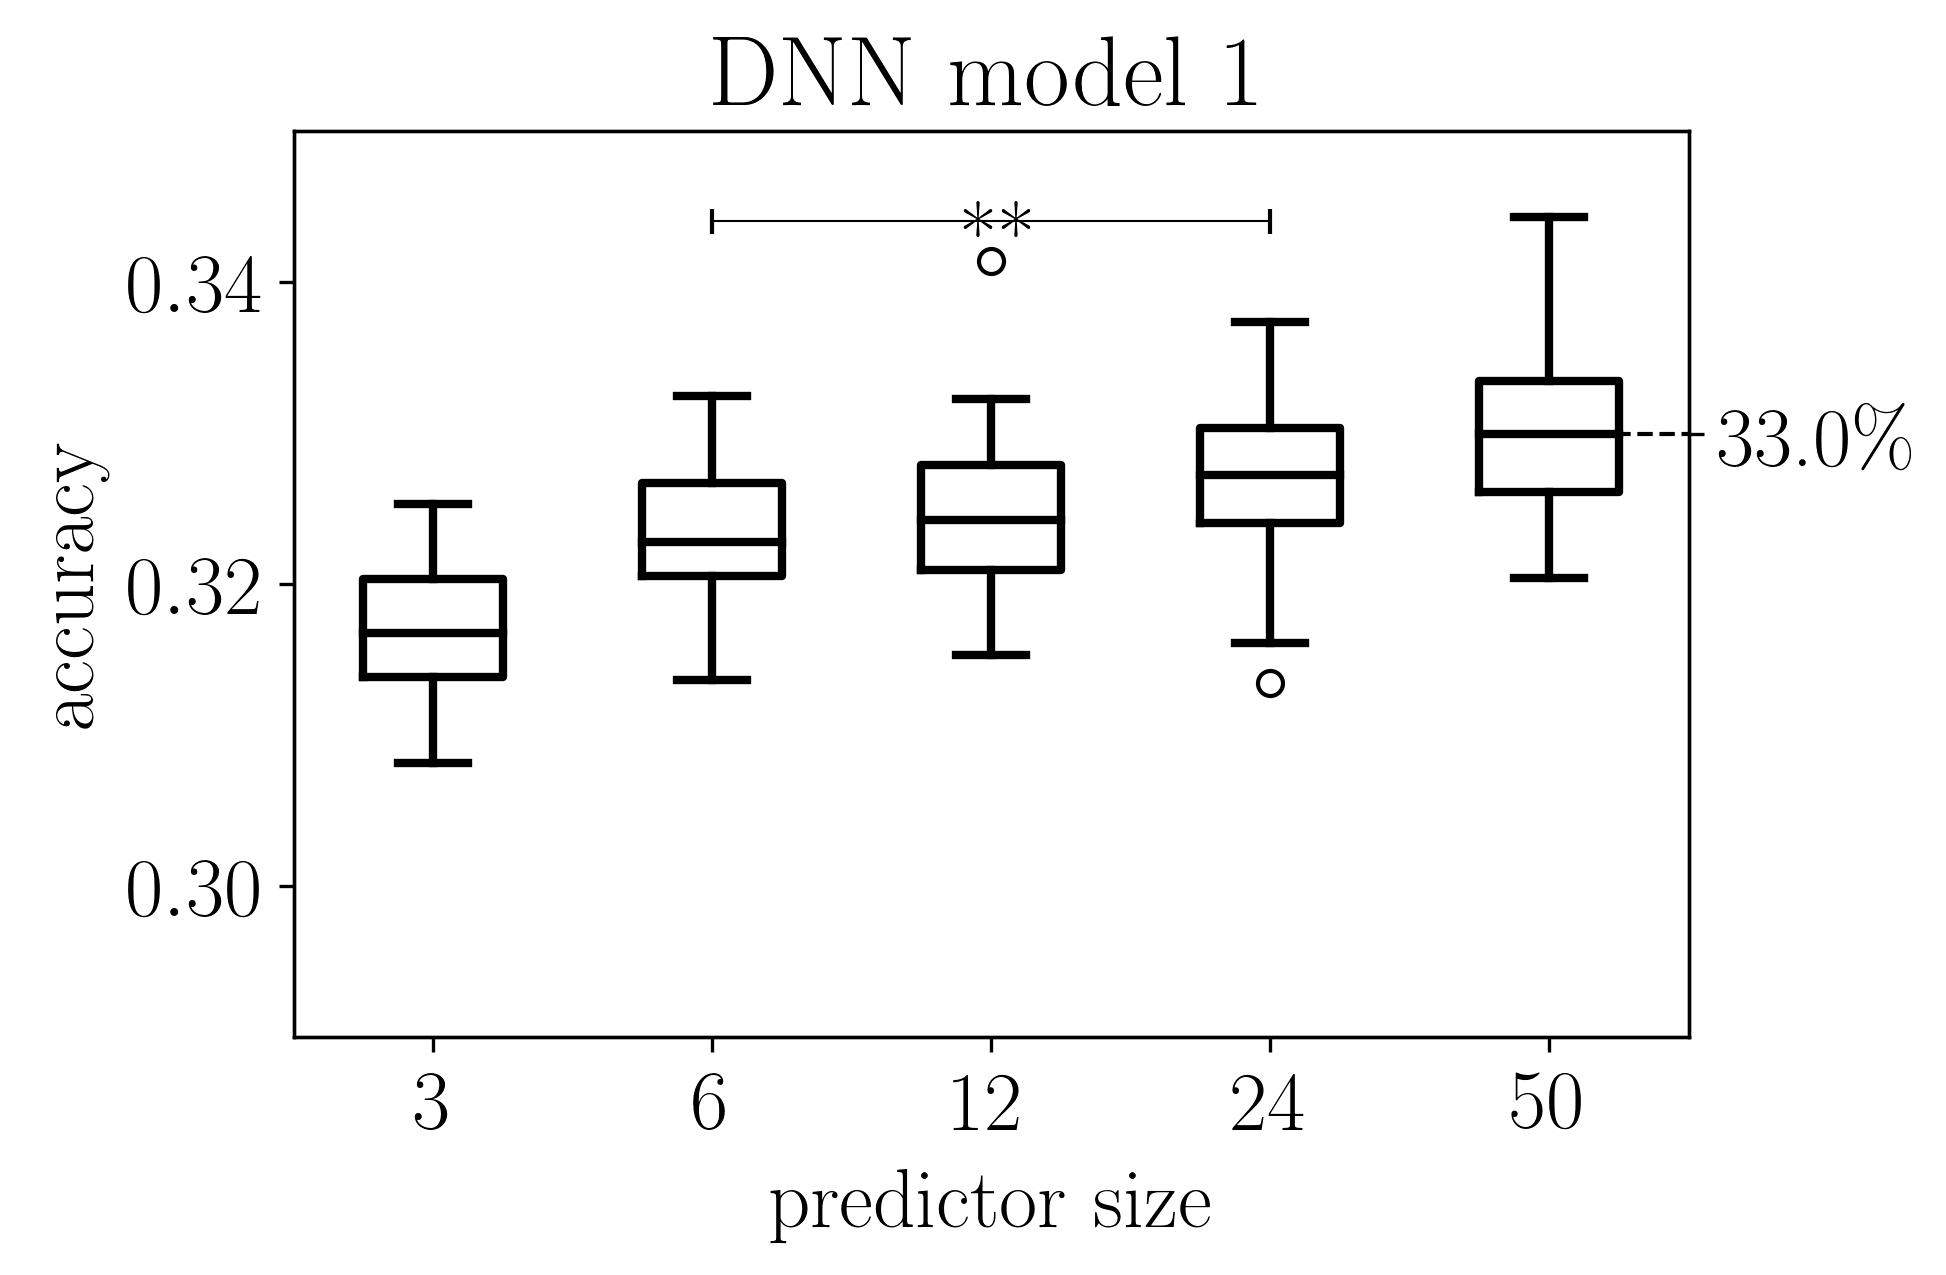
\includegraphics[width = \textwidth]{pics/dnn_model_1_all_runs_p1_ecoli_100000_10000_all_0.png}
		\label{fig:alpha}
	\end{subfigure}
	\begin{subfigure}[t]{0.48\linewidth}
%		\caption{mm}
		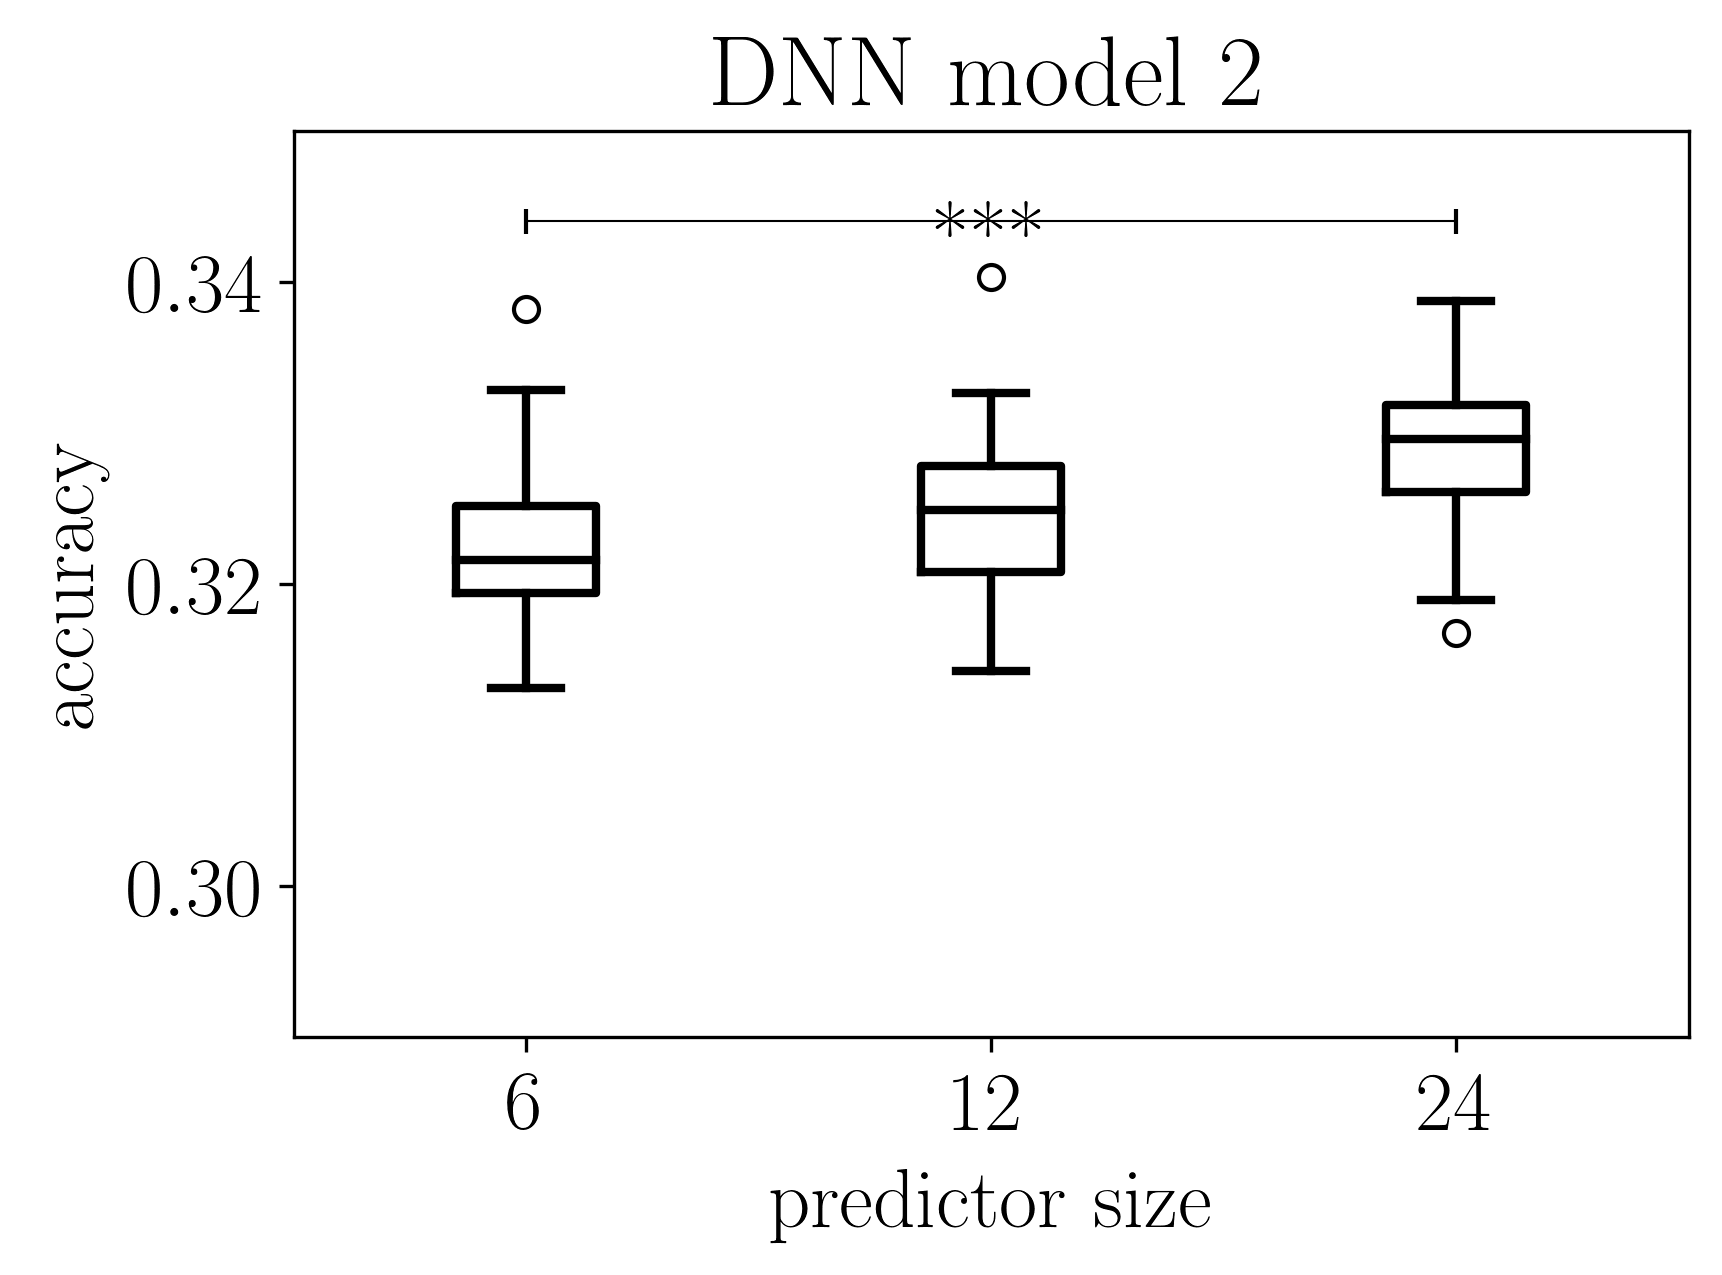
\includegraphics[width = \textwidth]{pics/dnn_model_2_all_runs_p1_ecoli_100000_10000_all_0.png}
			\label{fig:alpha}
	\end{subfigure}
	\begin{subfigure}[]{0.48\linewidth}
%		\caption{{\bfseries CNN model 1} \\* Сверточная однослойная модель }
		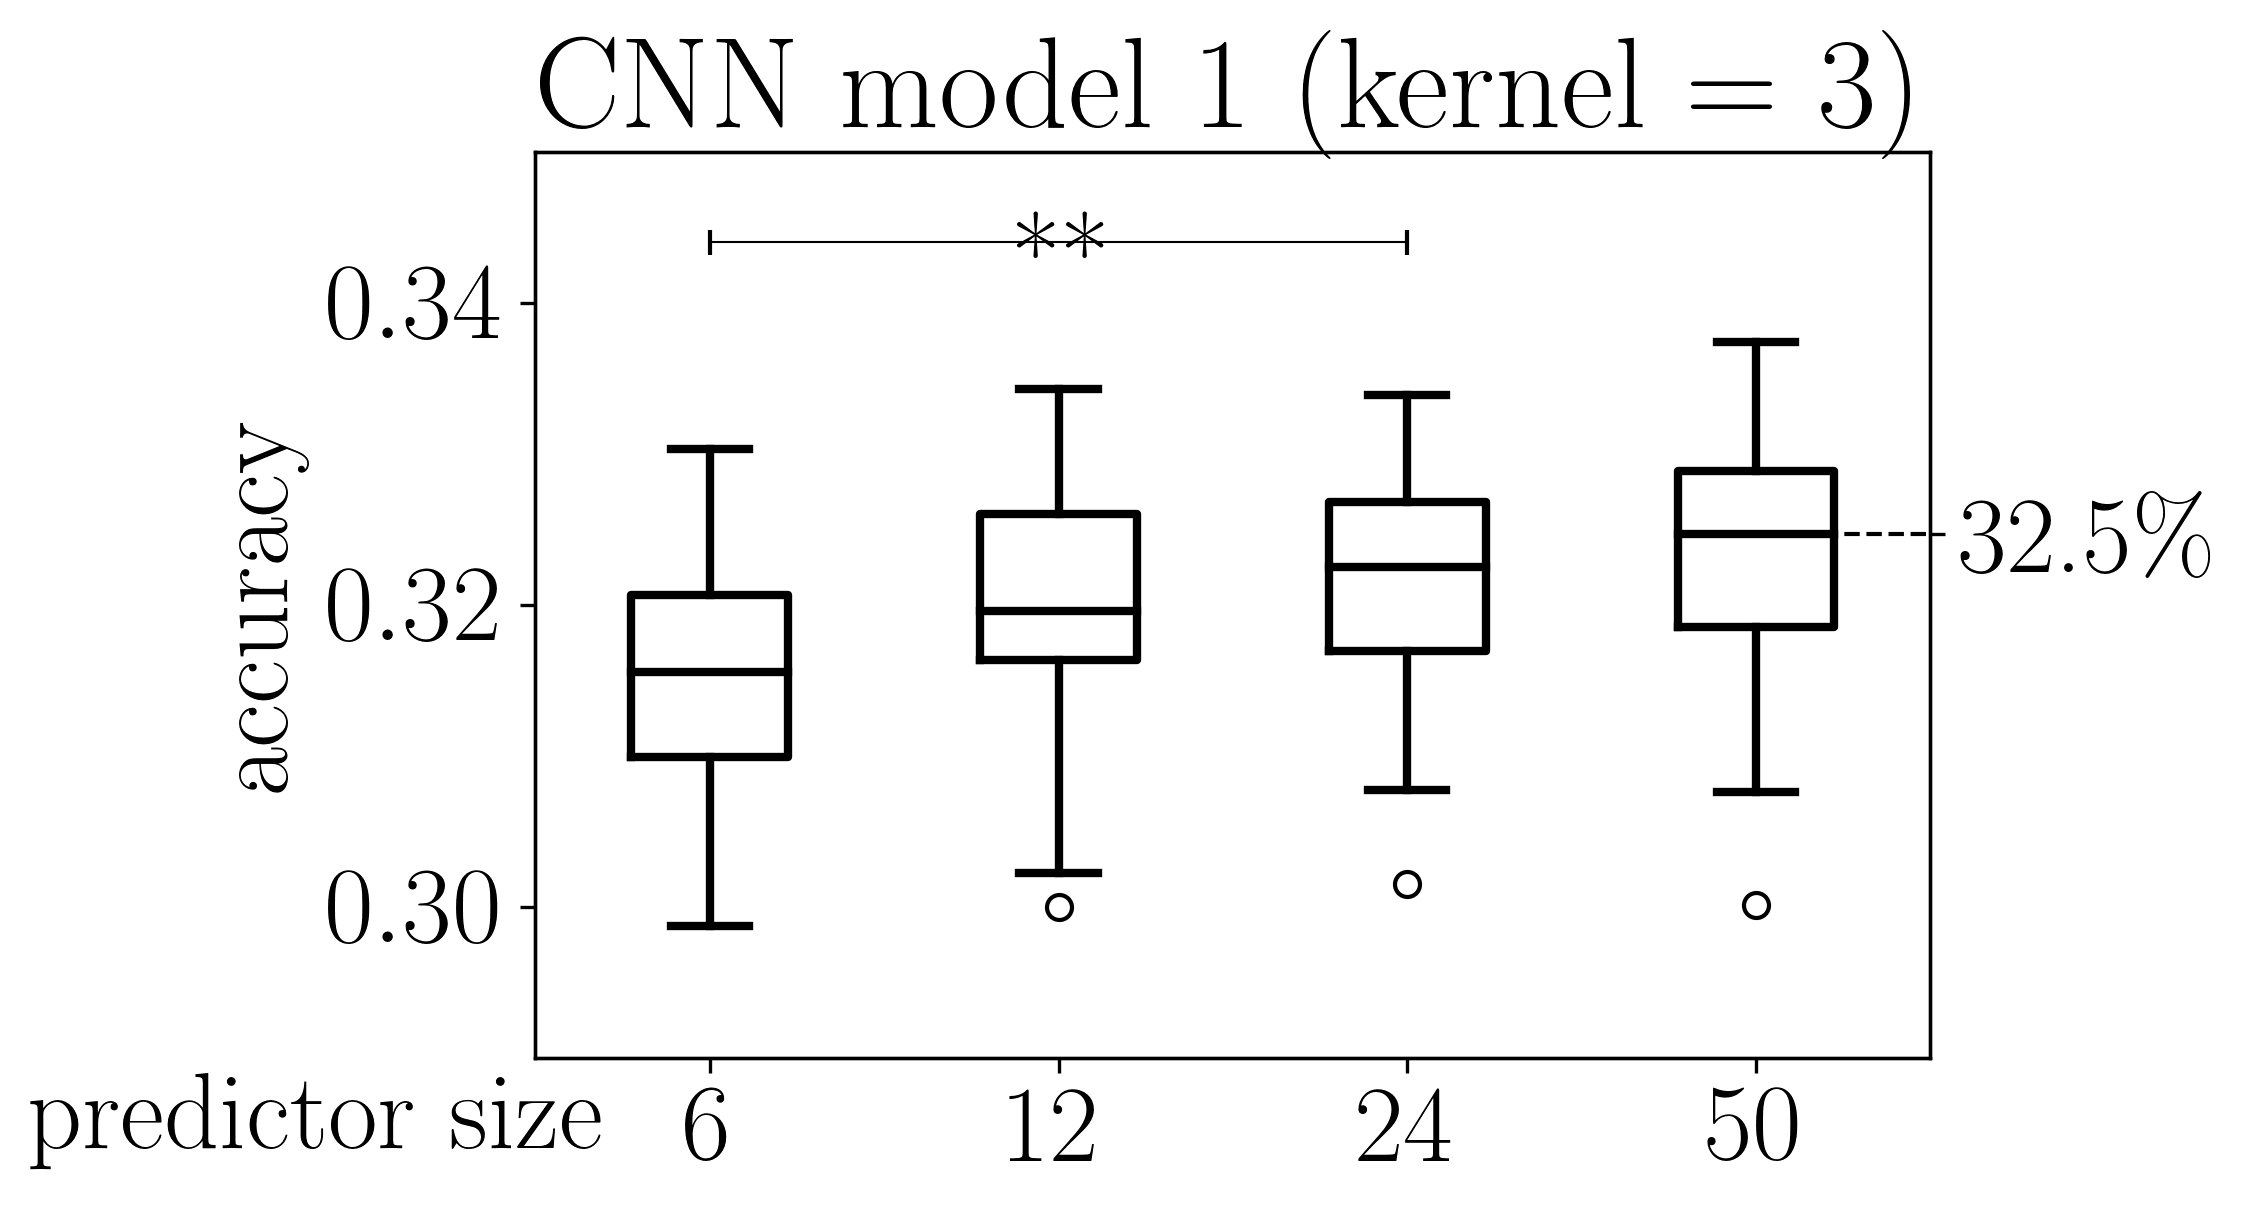
\includegraphics[width = \textwidth]{pics/cnn_model_1_all_runs_p1_ecoli_100000_10000_all_0.png}
		\label{fig:beta}
	\end{subfigure}
	\begin{subfigure}[]{0.48\linewidth}
%		\caption{{\bfseries CNN model 1} \\* Сверточная однослойная модель }
		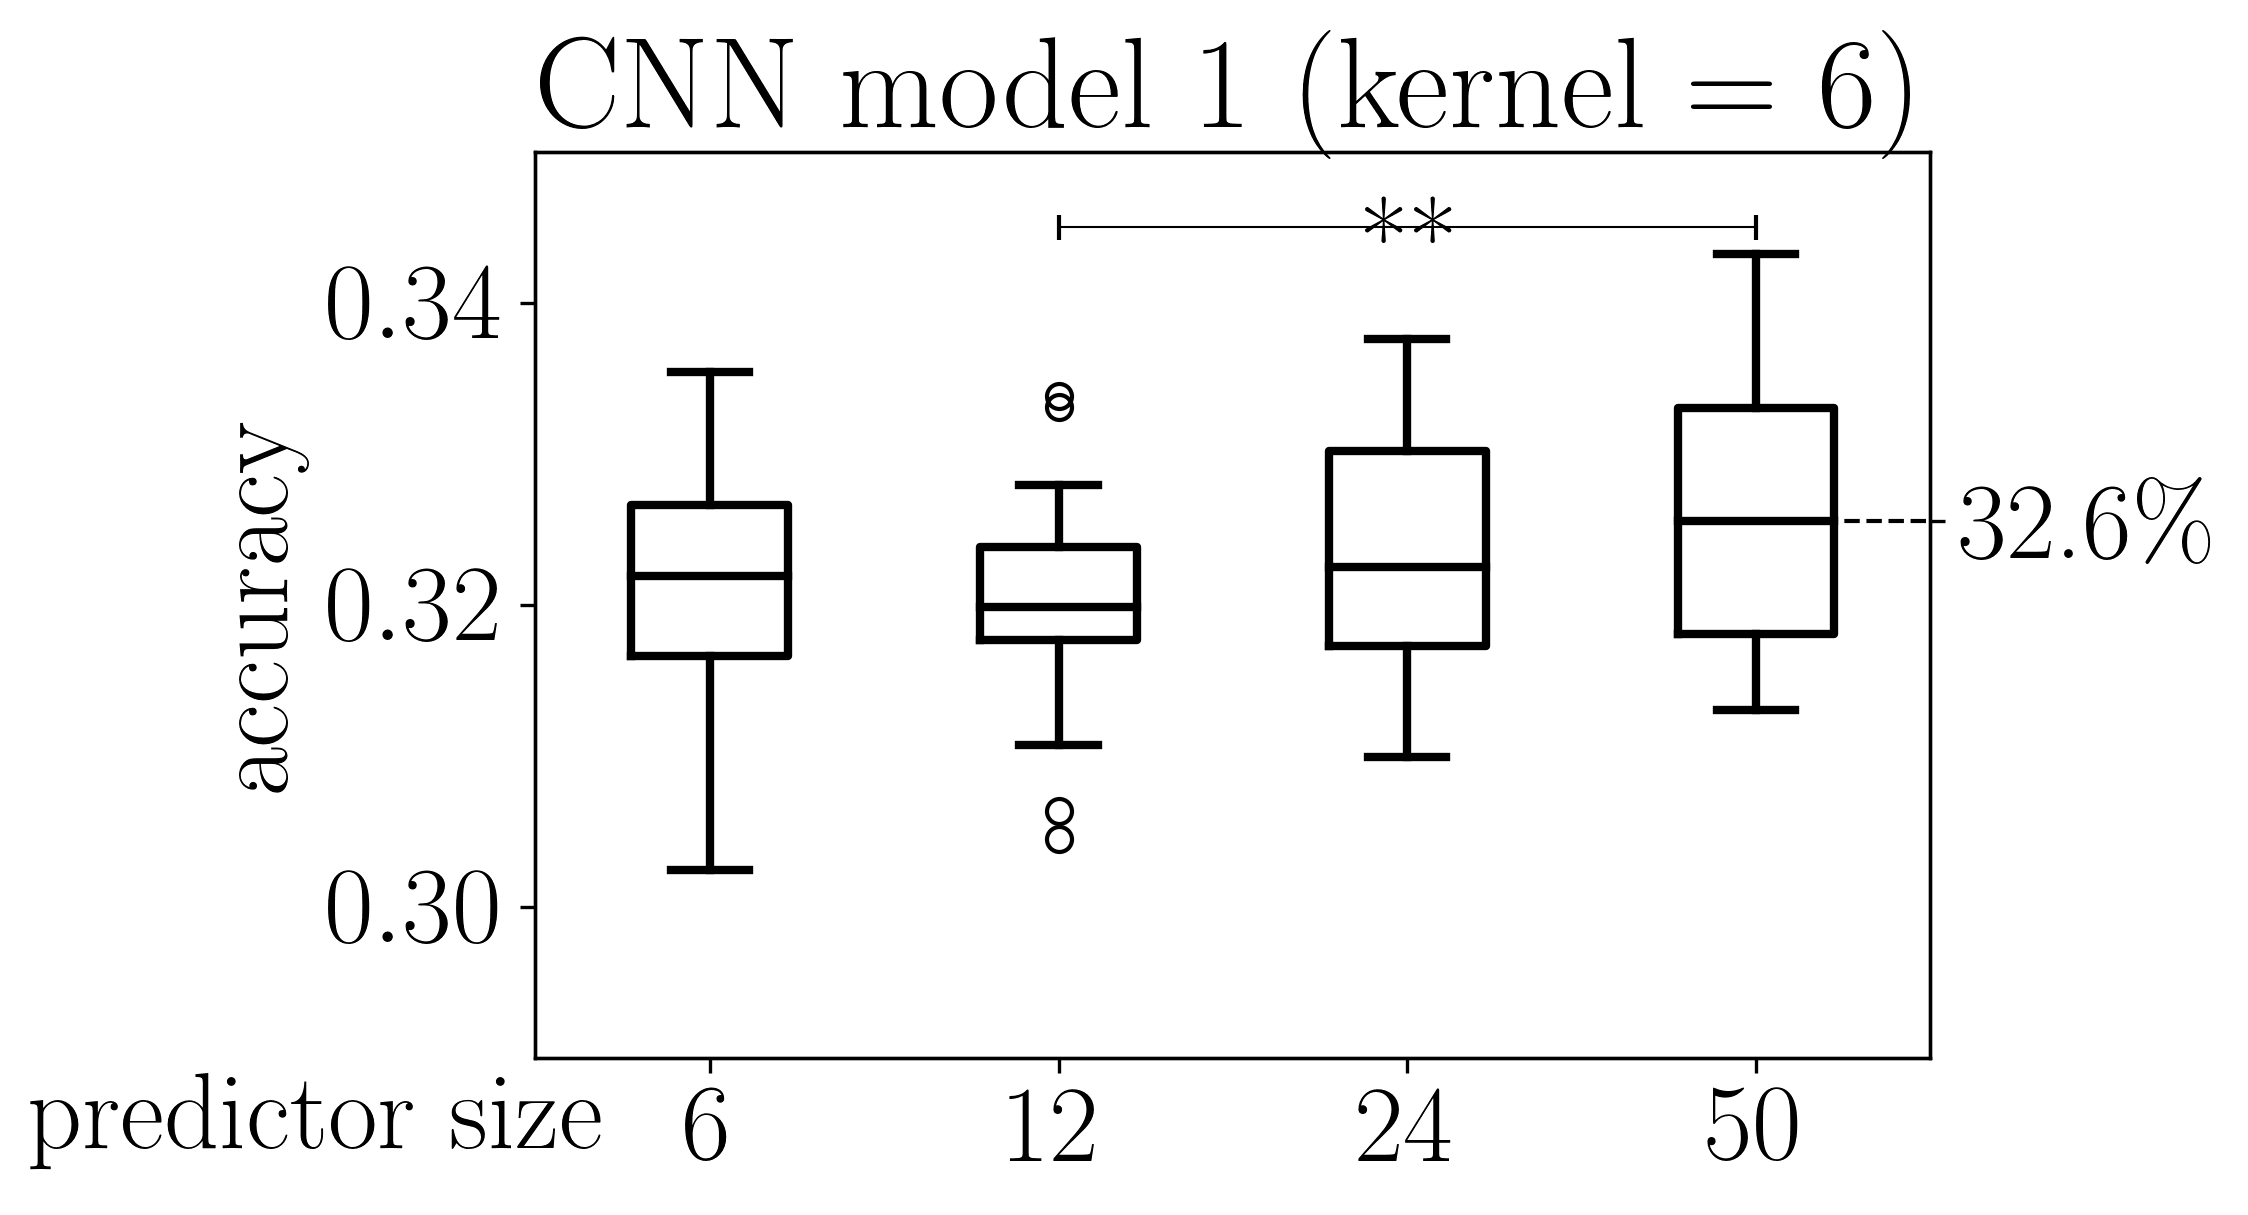
\includegraphics[width = \textwidth]{pics/cnn_model_2_all_runs_p1_ecoli_100000_10000_all_0.png}
		\label{fig:cnn_2_predictor}
	\end{subfigure}
	\caption{{\bfseries Зависимость точности предсказания от размера предикторной области для различных архитектур.} \\*
	По горизонтальной оси обозначен размер области. По вертикальной оси показано распределение точностей обученной модели в сете из 30 запусков с различными наборами данных.}
	
	\label{fig:size}
	
\end{figure*}

\paragraph{Зависимость от отступа.} Была исследована зависимость качества предсказания от расстояния между предикторной областью и предсказываемым нуклеотидом для двух моделей -- полносвязной и сверточной. 

С увеличением отступа качество предсказания падает, причем резко. Это подтверждает то, что в простых моделях (полносвязных и сверточных с небольшим числом параметров) предсказание основывается на ближайших в предсказываемому нуклеотидах.

\begin{figure*}[h] % two pictures
	\centering
	\begin{subfigure}[t]{0.47\linewidth}
		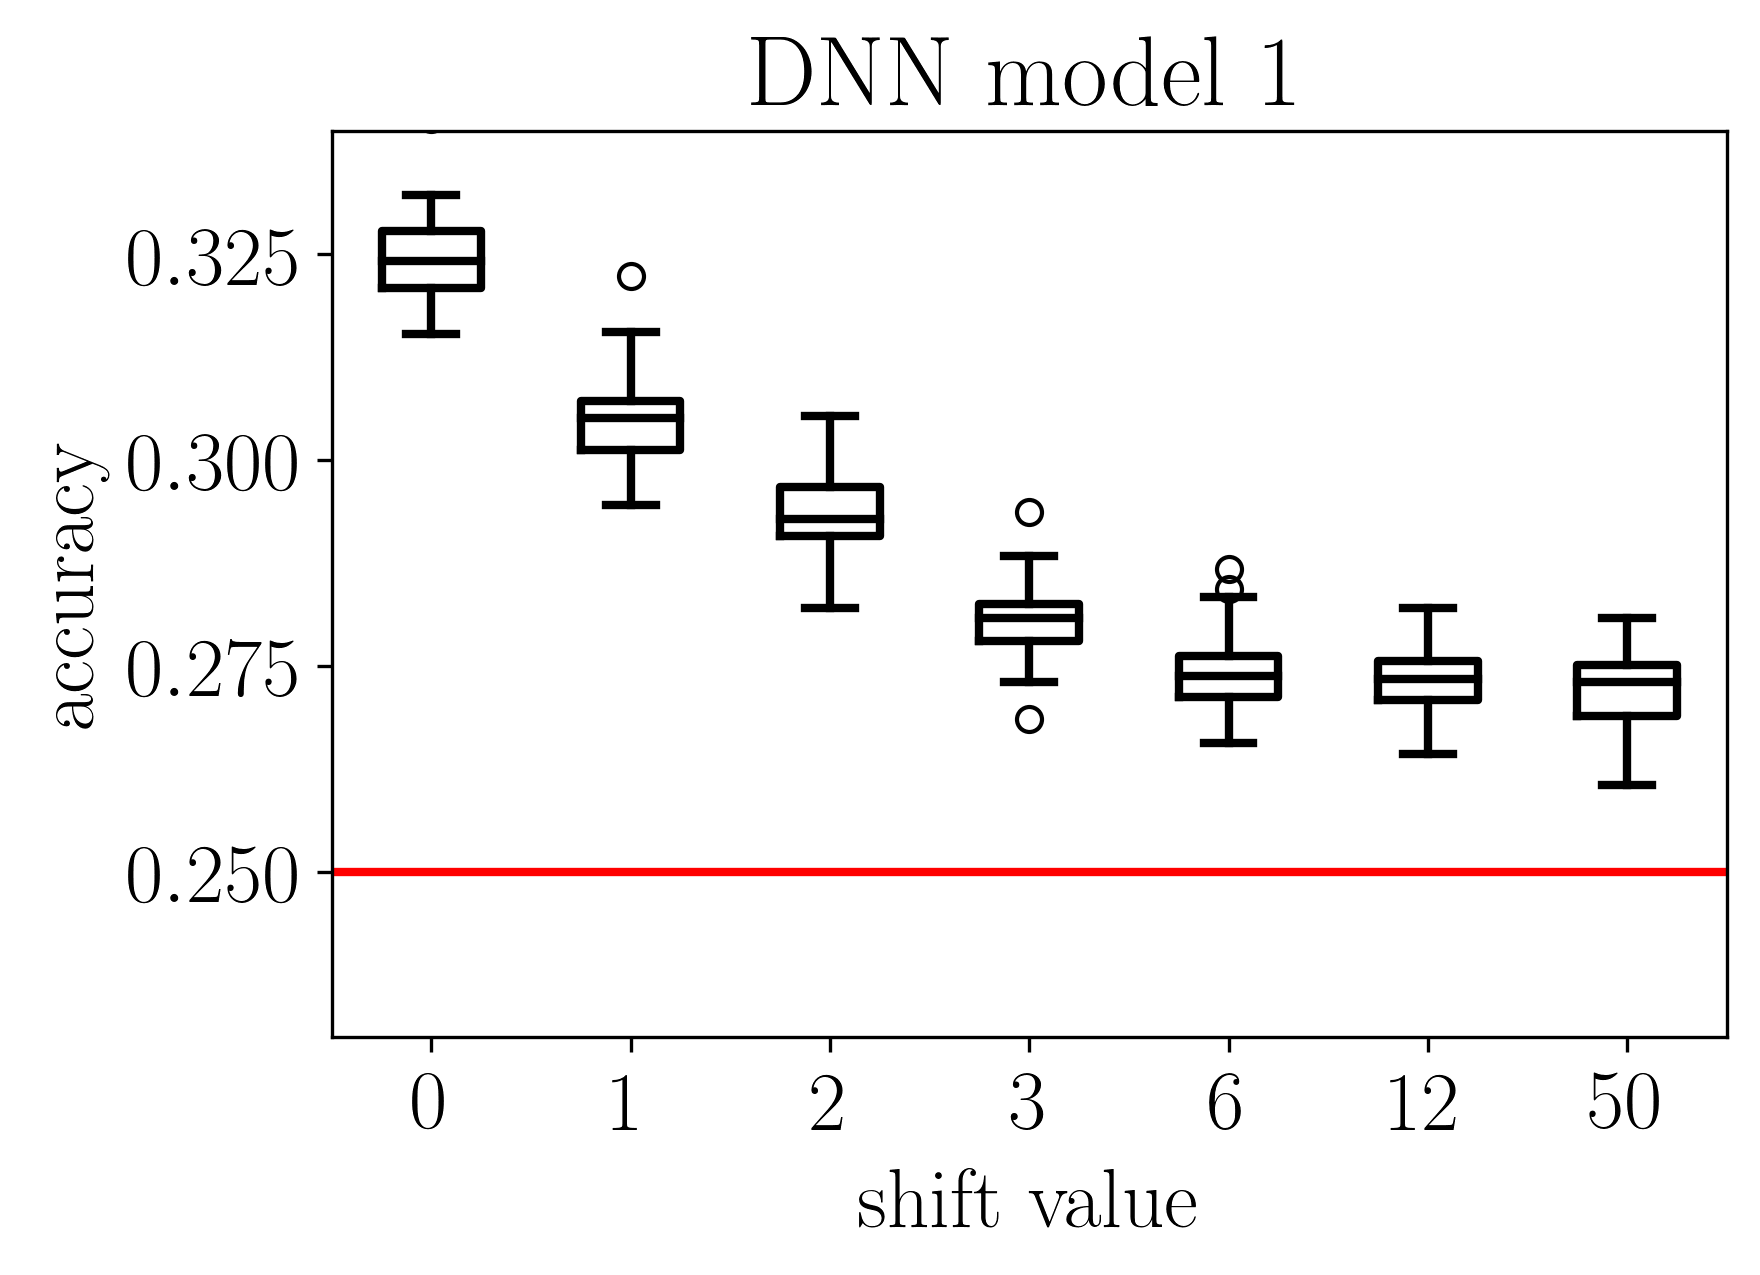
\includegraphics[width = \textwidth]{pics/dnn_model_1_all_runs_p1_ecoli_100000_10000_12_all.png}
		\caption{{\bfseries DNN model 1} \\*
		Полносвязная однослойная модель. Размер предикторной области 12.
		}
		\label{fig:dnn_shift}
	\end{subfigure}
	\begin{subfigure}[t]{0.47\linewidth}
		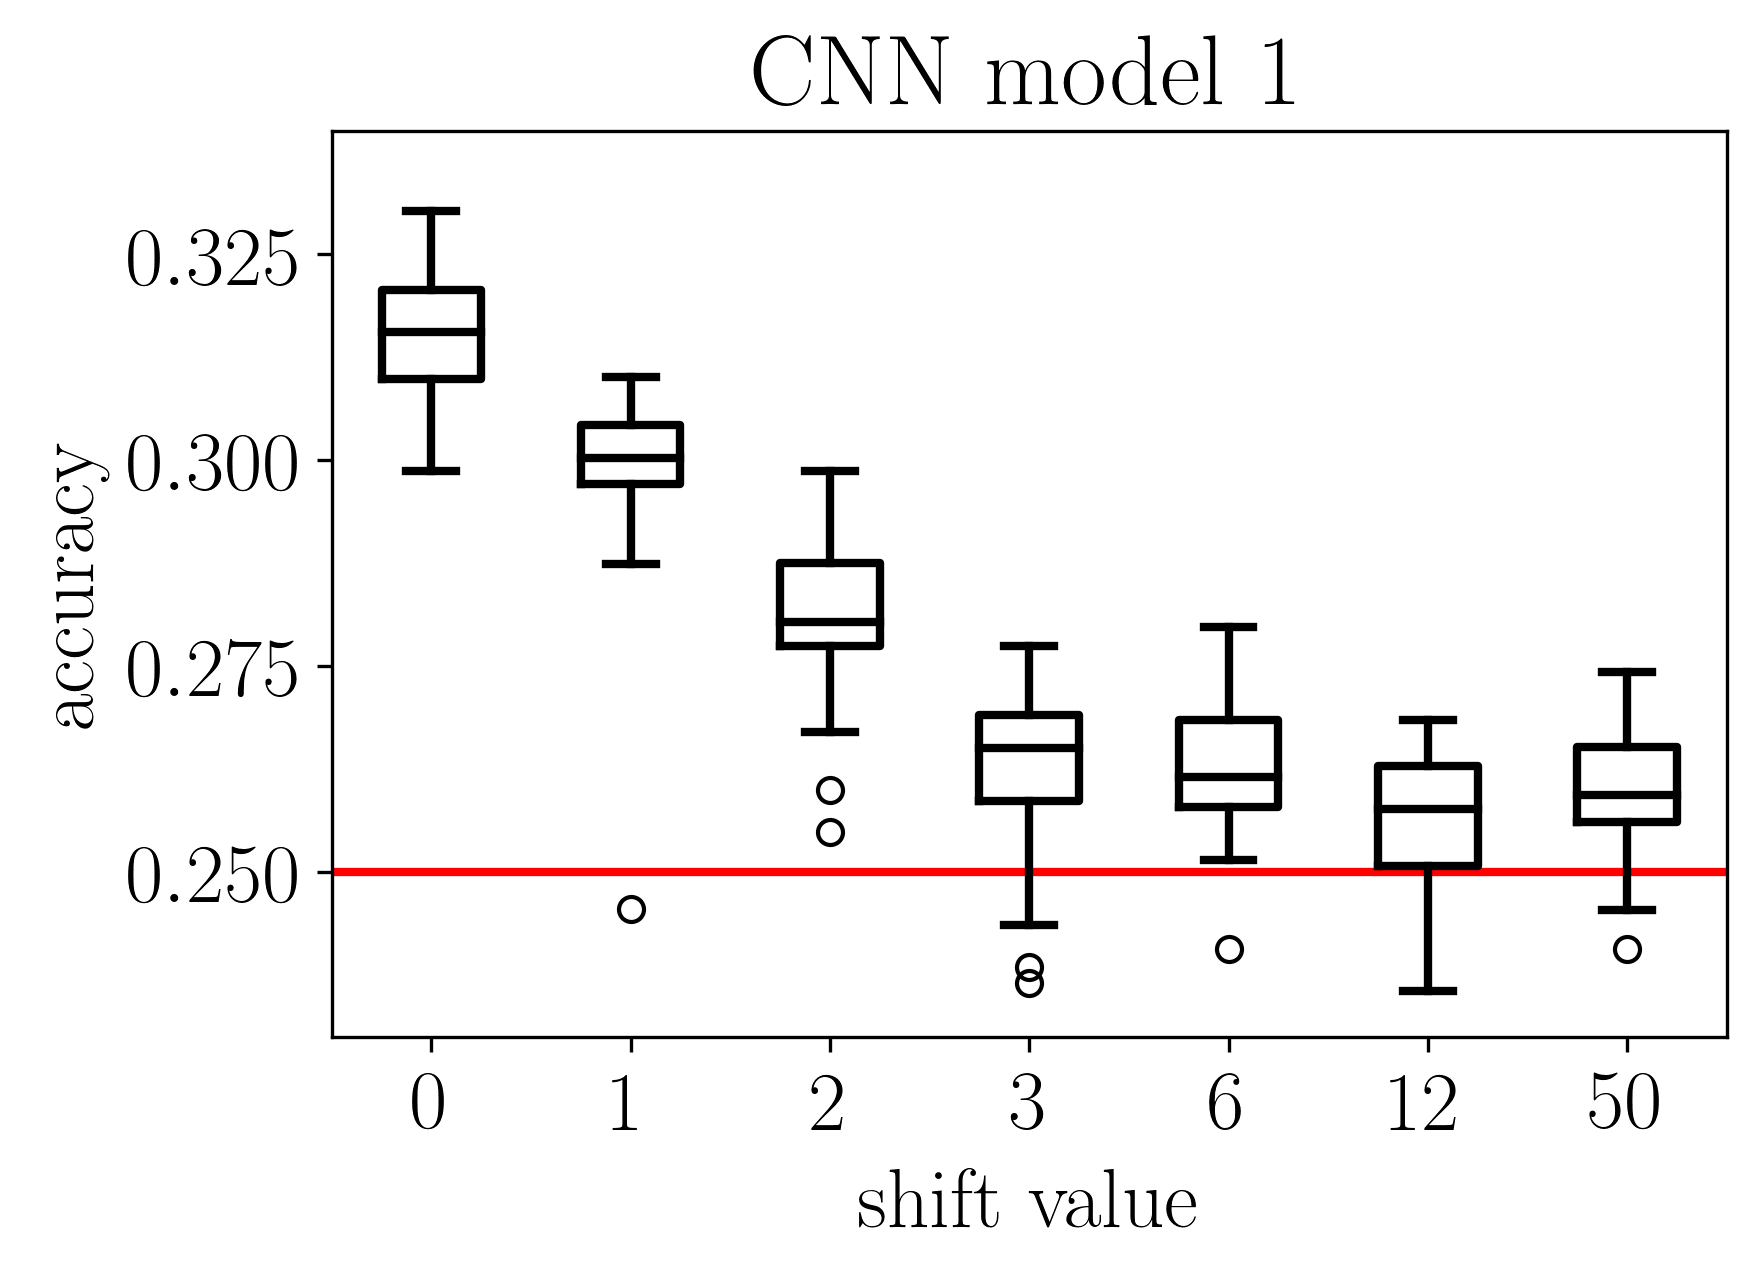
\includegraphics[width = \textwidth]{pics/cnn_model_1_all_runs_p1_ecoli_100000_10000_6_all.png}
		\caption{{\bfseries CNN model 1 (kernel = 3)} \\*
		Сверточная однослойная модель. Размер предикторной области 6.
		}
		\label{fig:cnn_shift}
	\end{subfigure}
	\caption{{\bfseries Зависимость точности предсказания от расстояния между предикторной областью и предсказываемым нуклеотидом (от отступа)  для различных архитектур.} \\*
	По горизонтальной оси обозначен размер отступа. По вертикальной оси показано распределение точностей обученной модели в 30 запусках с различными наборами данных. Горизонтальная линия отмечает точность случайного предсказания 25\%.}	
	\label{fig:shift}
	
\end{figure*}
 
 \paragraph{Сравнение полносвязных моделей.} Мы сравнили между собой полносвязные модели -- с одним (DNN model 1) и двумя слоями (DNN model 2)  на двух типах данных -- предсказание по предикторной области 12 и 24 (рисунок \ref{fig:dnn_test}). Статистически значимой разницы между моделями не наблюдалось.
 
 Полносвязные модели по построению не могут должным образом использовать информацию о расположении и последовательности нуклеотидов, так как входниые переменные -- нуклеотиды -- независимы для сети. В таких моделях предсказание, в большей степени, основывается на нуклеотидном составе предикторной области.
 
\begin{figure}[h] % picture
	\centering
	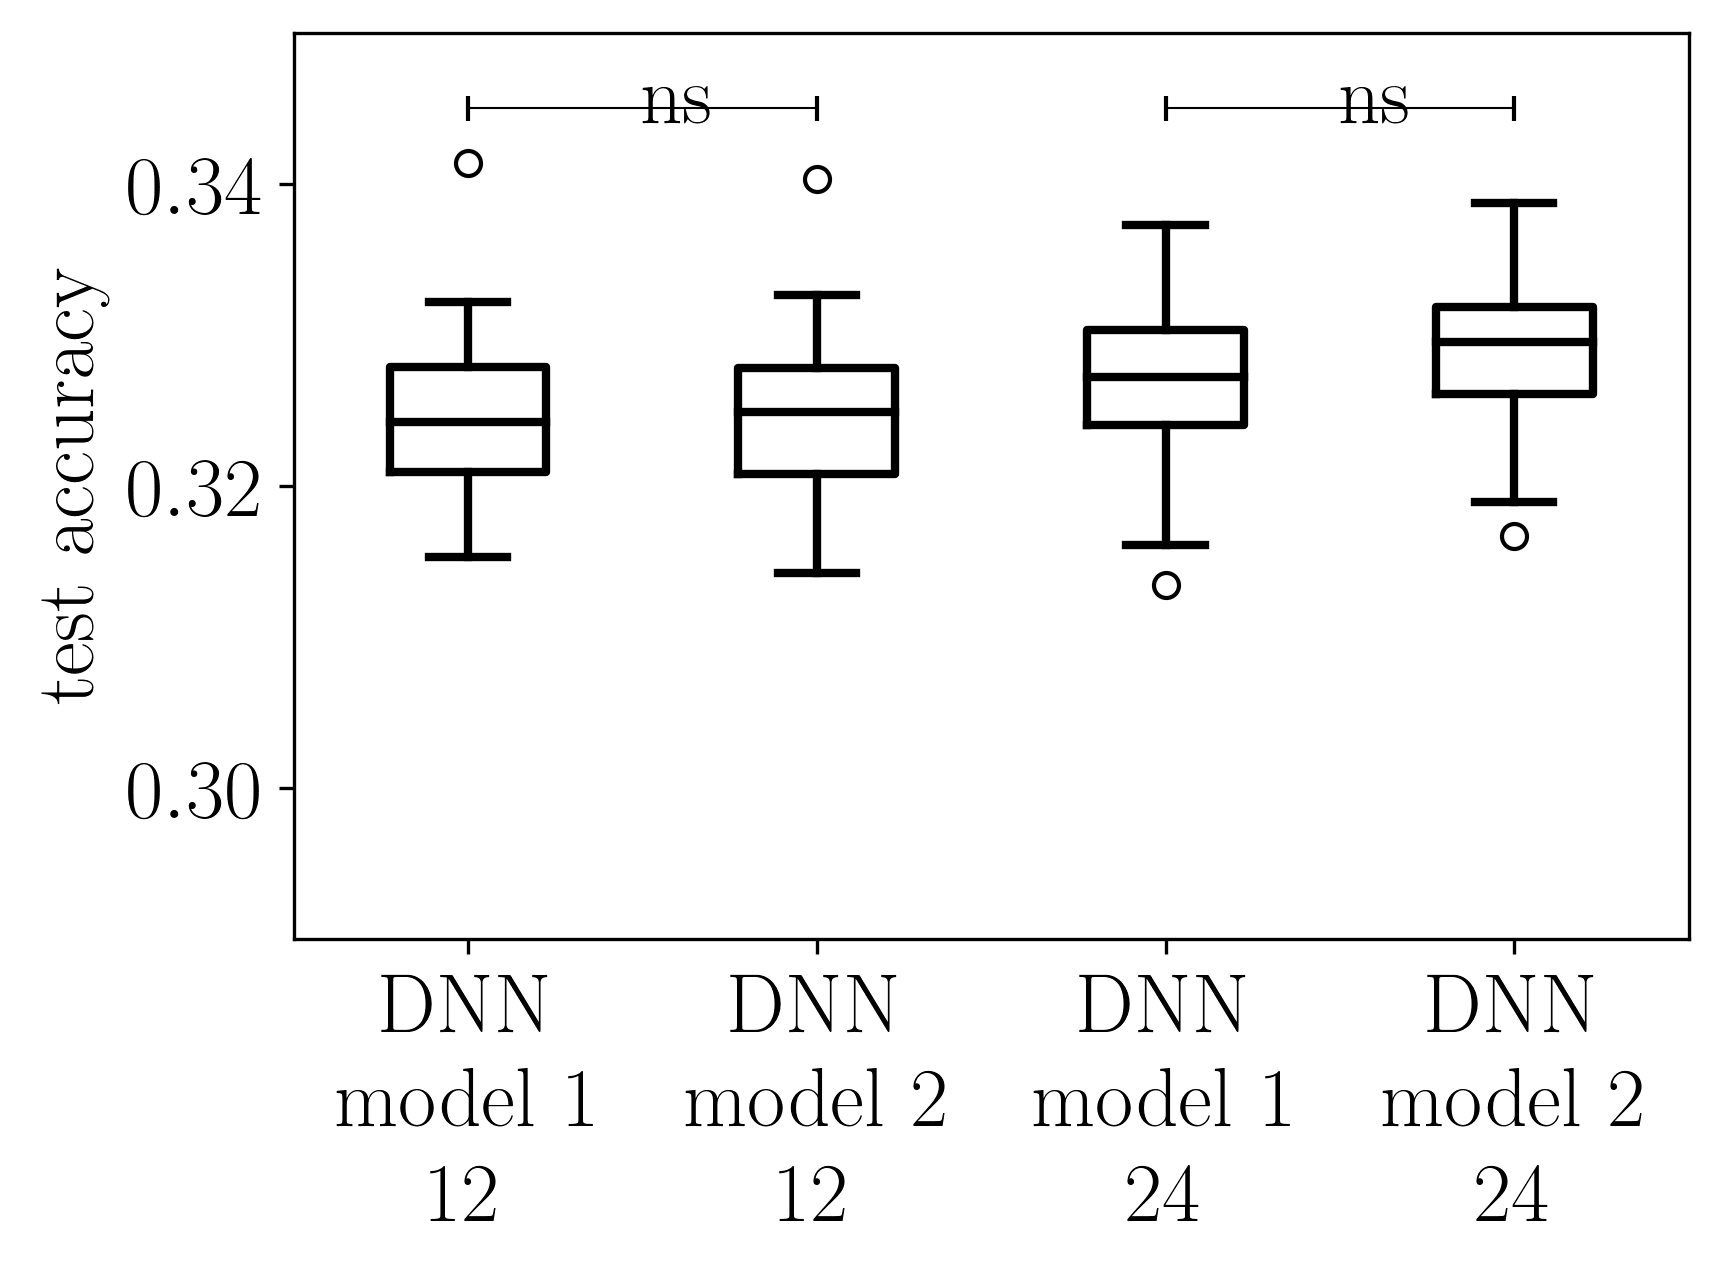
\includegraphics[width = 0.6\textwidth]{pics/dnn_models_all_runs_p1_ecoli_100000_10000_12_0.png}
	\caption{{\bfseries Сравнение полносвязных моделей.} \\* 
		На рисунке показано распределение качестве предсказания полносвязных моделей на двух вариантах данных -- с предикторной областью 12 и 24. В обоих случаях разница в качестве предсказания статистически не значима. \\
		   \mannwhitni }
	\label{fig:dnn_test}	
\end{figure}


\paragraph{Сверточные модели.} Сверточные модели были протестированы на пресказание по левой предикторной области. Мы исследовали зависимость предсказания от конфигурации сверточного слоя в простейшей модели. Результаты тестов приведены на рисунке \ref{fig:cnn_test}.

Увеличение размера сверточного фильтра с 3 до 6 не дает значительного прироста точности. При этом увеличение количества фильтров дает значительное увеличение точности, так как позволяет распознавать больше паттернов в последовательности \ref{fig:cnn_test1}.

ВЫВОД ПРО ИСПОЛЬЗОВАНИЕ STRIDE	

Также на простейших сверточных моделях мы сравнили, выше ли точность при обучении и предсказании с использованием только кодирующих контекстов, то есть выбранных из кодирующих частей генома. Использование кодирующих контекстов дало значительный, но небольшой прирост в точности для всех проверенных моделей \ref{fig:cnn_test2}. 

\input{tables/cnn_comparison}


\paragraph{Рекурретные модели.}
Мы протестировали рекуррентные модели, состоящие из одного LSTM слоя с разным числом скрытых состояний и одного решающего полносвязного слоя.
С увеличением числа скрытых слоев точность предсказания растет \ref{fig:rnn_test}.

Однако обучение рекуррентных моделей не поддается вычислительному распараллеливанию, что делает такие задачи очень долгоими для вычиления. время обучения простейшей рекуррентной модели в разы превышает время обучения сверточной модели.  

\begin{figure}[H] % picture
	\centering
	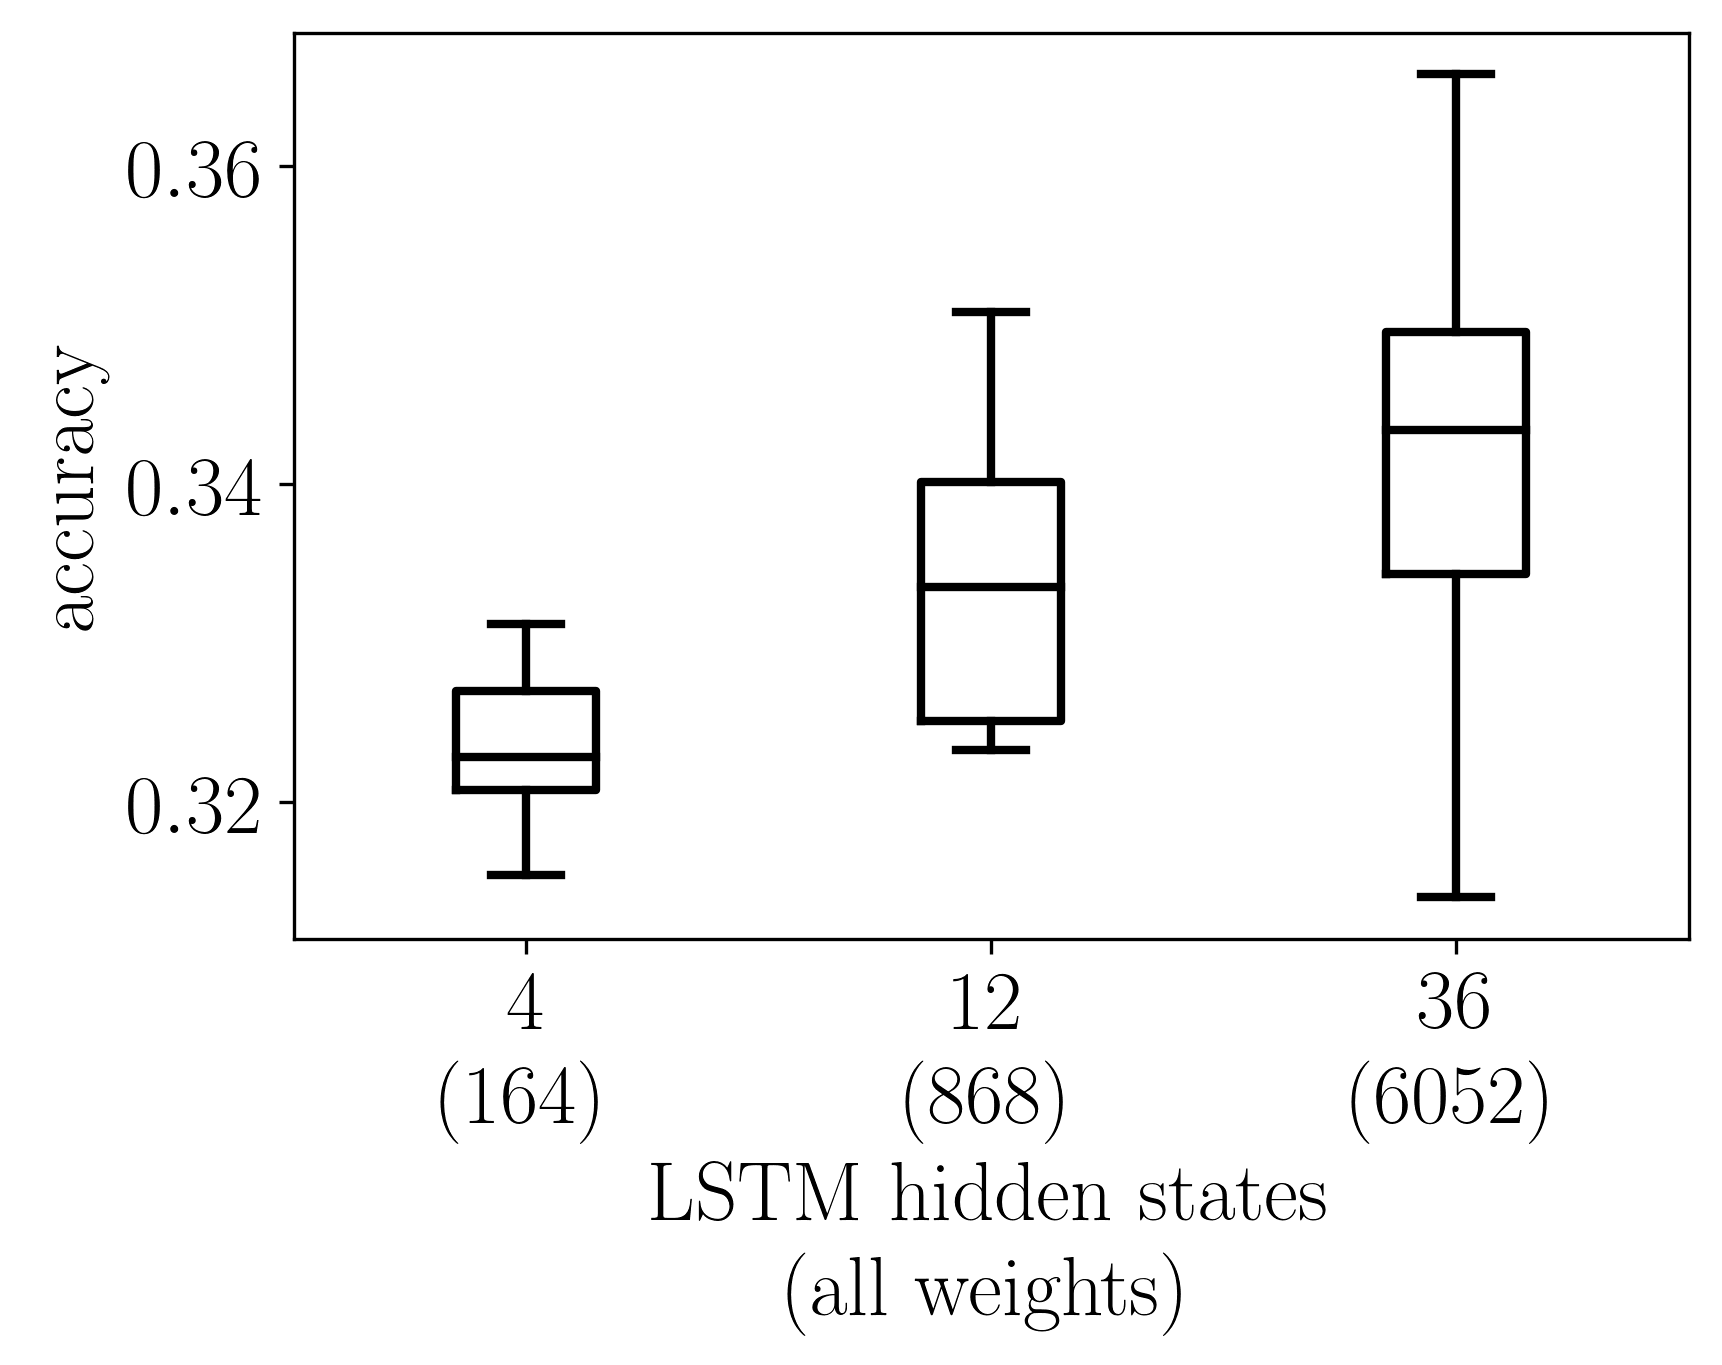
\includegraphics[width = 0.6\textwidth]{pics/rnn_models_all_runs_p1_ecoli_100000_10000_50_0.png}
	\caption{{\bfseries Сравнение рекуррентных моделей.} \\* 
		   \mannwhitni }
	\label{fig:rnn_test}	
\end{figure}

\paragraph{Использование двустроннего контекста.} Для более эффективного предсказания мы протестировали архитектуры сверточных нейронных сетей, которые учитывают контекст с двух сторон от нуклеотида. 

Использование нуклеотидного контекста с двух сторон в сверточных моделях показало наилучшую точность.

\begin{figure}[H] % picture
	\centering
	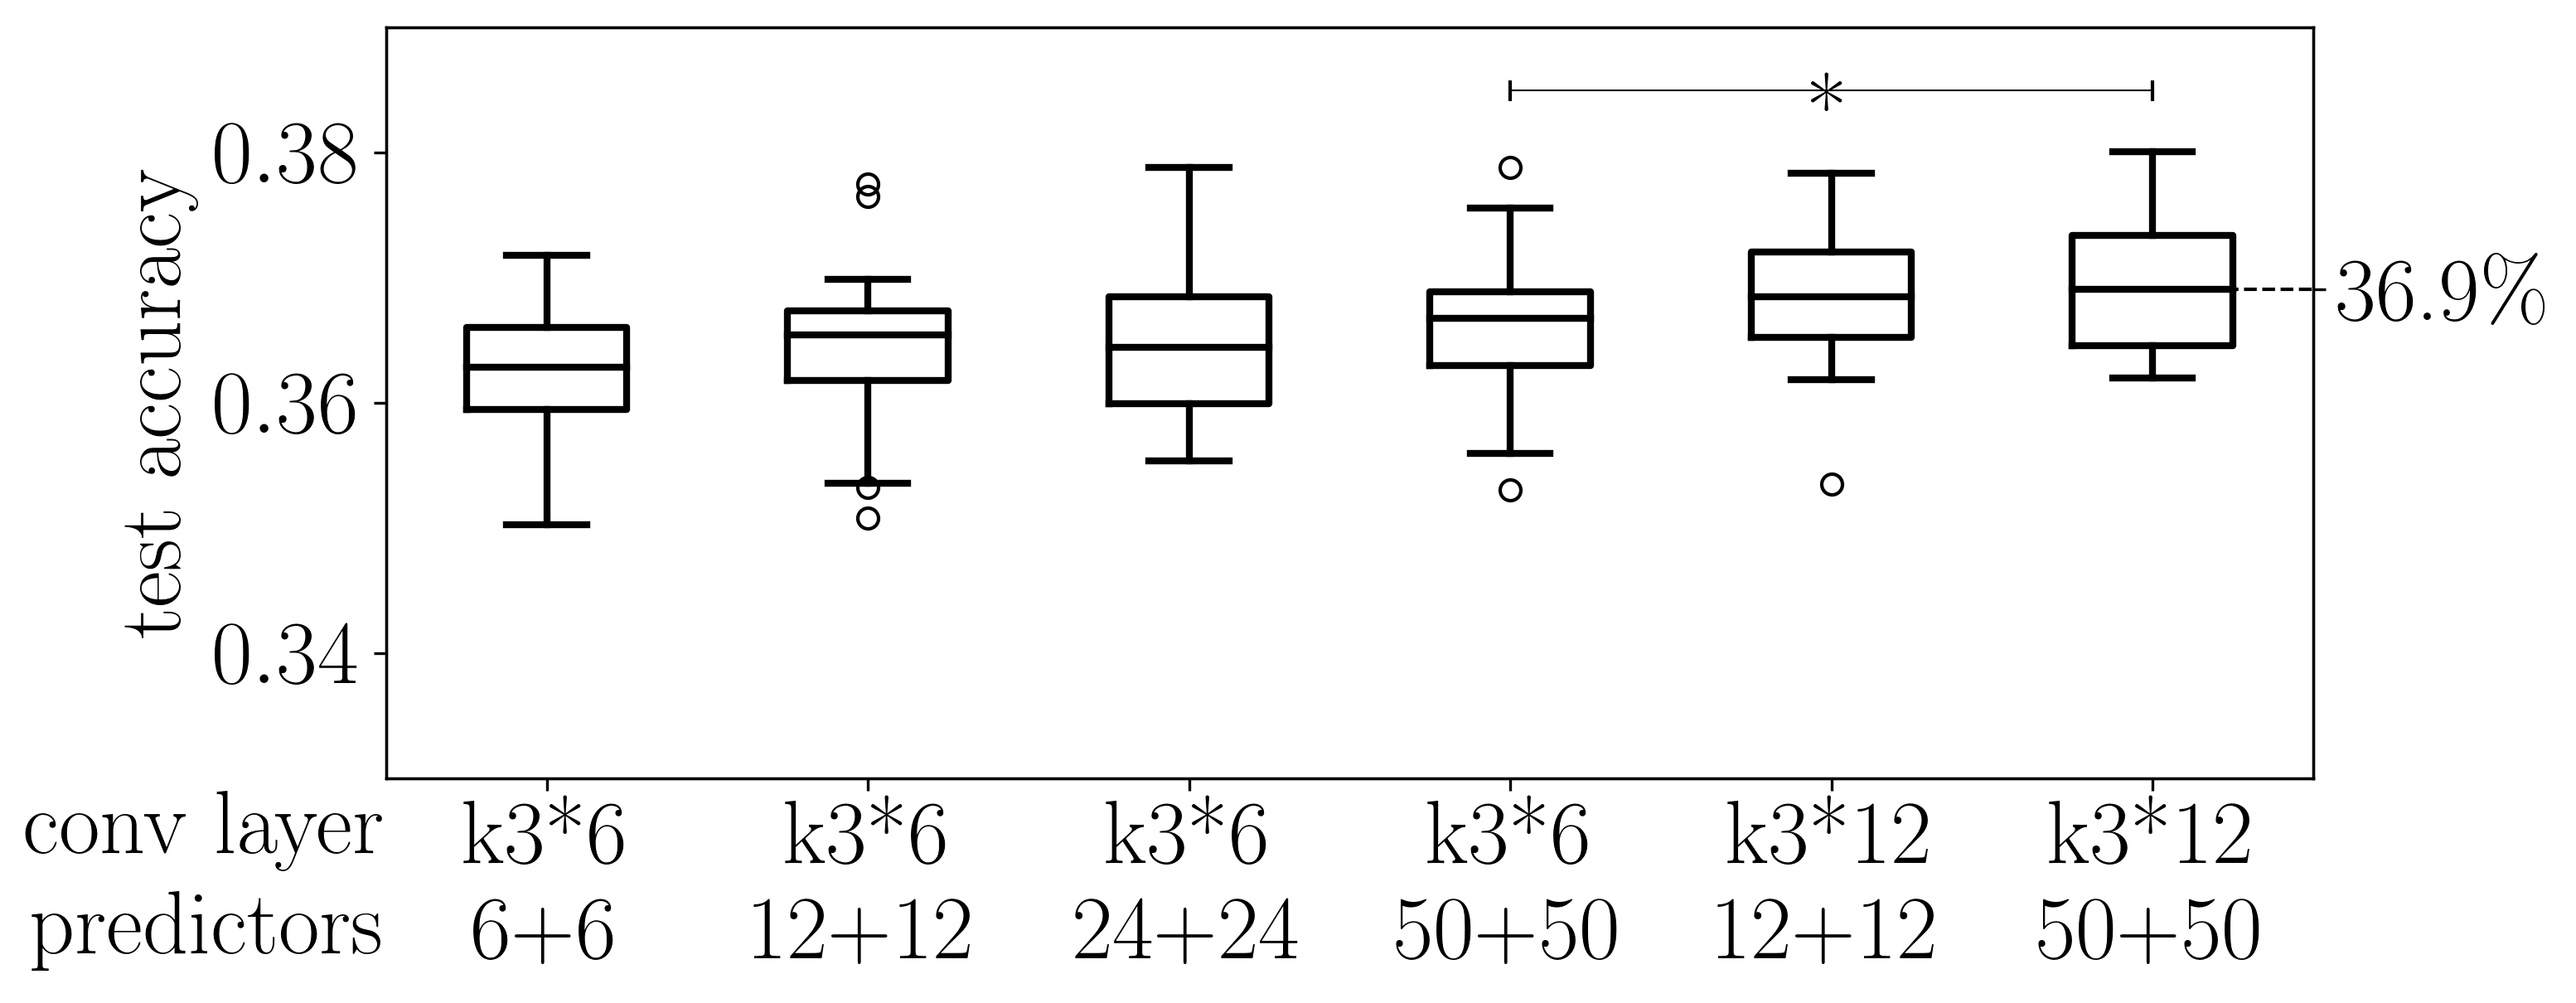
\includegraphics[width = 0.6\textwidth]{pics/cnn_models_two_sided.png}
	\caption{{\bfseries} Сравнение сверточных моделей при использовании контекста с двух сторон.\\* }
	\label{fig:cnn_twosided}	
\end{figure}
	 \newpage
%        %
%\begin{figure}[h] % picture
%	\centering
%	\includegraphics[width = 0.1\textwidth]{}
%	\caption{caption}
%	\label{fig:plasmid}	
%\end{figure}
%
%
%
%\begin{figure*}[h] % two pictures
%	\centering
%	\begin{subfigure}[t]{0.1\linewidth}
%		\includegraphics[width = \textwidth]{}
%		\caption{caption 1}\label{fig:alpha}
%	\end{subfigure}
%	\begin{subfigure}[t]{0.1\linewidth}
%		\includegraphics[width = \textwidth]{}
%		\caption{caption 2}\label{fig:beta}
%
%	\end{subfigure}
%	\caption{great caption}
%	\label{fig:structs}
%	
%\end{figure*}
%
%
%
%\begin{table}[p]
%	\small
%	\caption{caption}
%	\label{table:strains}
%	\begin{tabular}{ p p p }
%
%		Название штамма & Описание & Источник \\ 
%
%		W303 & MAT\textbf{a} ade2-101 his3-11 trp1-1 ura3-52 can1-100 leu2-3,112, GAL, psi+ & $^1$ \\  
%
%
%		
%		блабла & блабал & jdsjf \\
%
%	\end{tabular}
%	
%\end{table}
%
%


        \footnotesize \bibliographystyle{mybib1.bst}  % стилевой файл для оформления по ГОСТу  utf8gost705u, ieeetr для курсовой, cell  -- черновик
        \bibliography{bib.bib}
\end{document}
